\chapter{METHODOLOGY}

\section{Methodological Overview}
This chapter presents a multi-stage, privacy-preserving computer vision framework to detect and count pediatric and adult persons in hospital outpatient waiting environments under heavy occlusion and variable lighting. The architecture integrates full-frame detection, secondary crop classification, and biological verification, as illustrated in Figure \ref{fig:system_arch}:
\begin{enumerate}[(i)]
    \item \textbf{Stage 1: Full-Frame Spatial Detection and Tracking:} Input video frames pass through Contrast Limited Adaptive Histogram Equalization (CLAHE) and Slicing Aided Hyper Inference (SAHI). A YOLO26s-ONNX detector predicts person bounding boxes. A ByteTrack tracker matches targets using an 8D Kalman filter, history-prioritized containment resolution, and anatomical seated occupant deduplication.
    \item \textbf{Stage 2: Margin-Expanded Crop Classification:} Candidate bounding boxes undergo margin expansion ($\alpha = 0.10$) and isotropic letterboxing to $224 \times 224$ pixels with neutral gray padding. A dedicated secondary ONNX crop classifier predicts raw demographic class probabilities.
    \item \textbf{Stage 3: Physical Prior and Temporal Consensus Fusion:} Raw model probabilities are modulated by a normalized height stature prior ($\theta_{\text{adult}} = 0.32$, $\theta_{\text{child}} = 0.20$) and smoothed across time via dual-horizon consensus weighting (70\% historical consensus and 30\% rolling window). Ambiguous detections are resolved using 17-point skeletal pose estimation to evaluate the cephalocaudal torso-to-leg growth ratio ($R_{\text{ceph}} = L_{\text{torso}} / L_{\text{leg}}$).
    \item \textbf{Cross-Camera Re-Identification Plugin:} An optional decoupled plugin extracts dual-zone upper and lower color signatures to link occupant trajectories across hospital rooms without cloud processing.
\end{enumerate}

\begin{figure}[htbp]
    \centering
    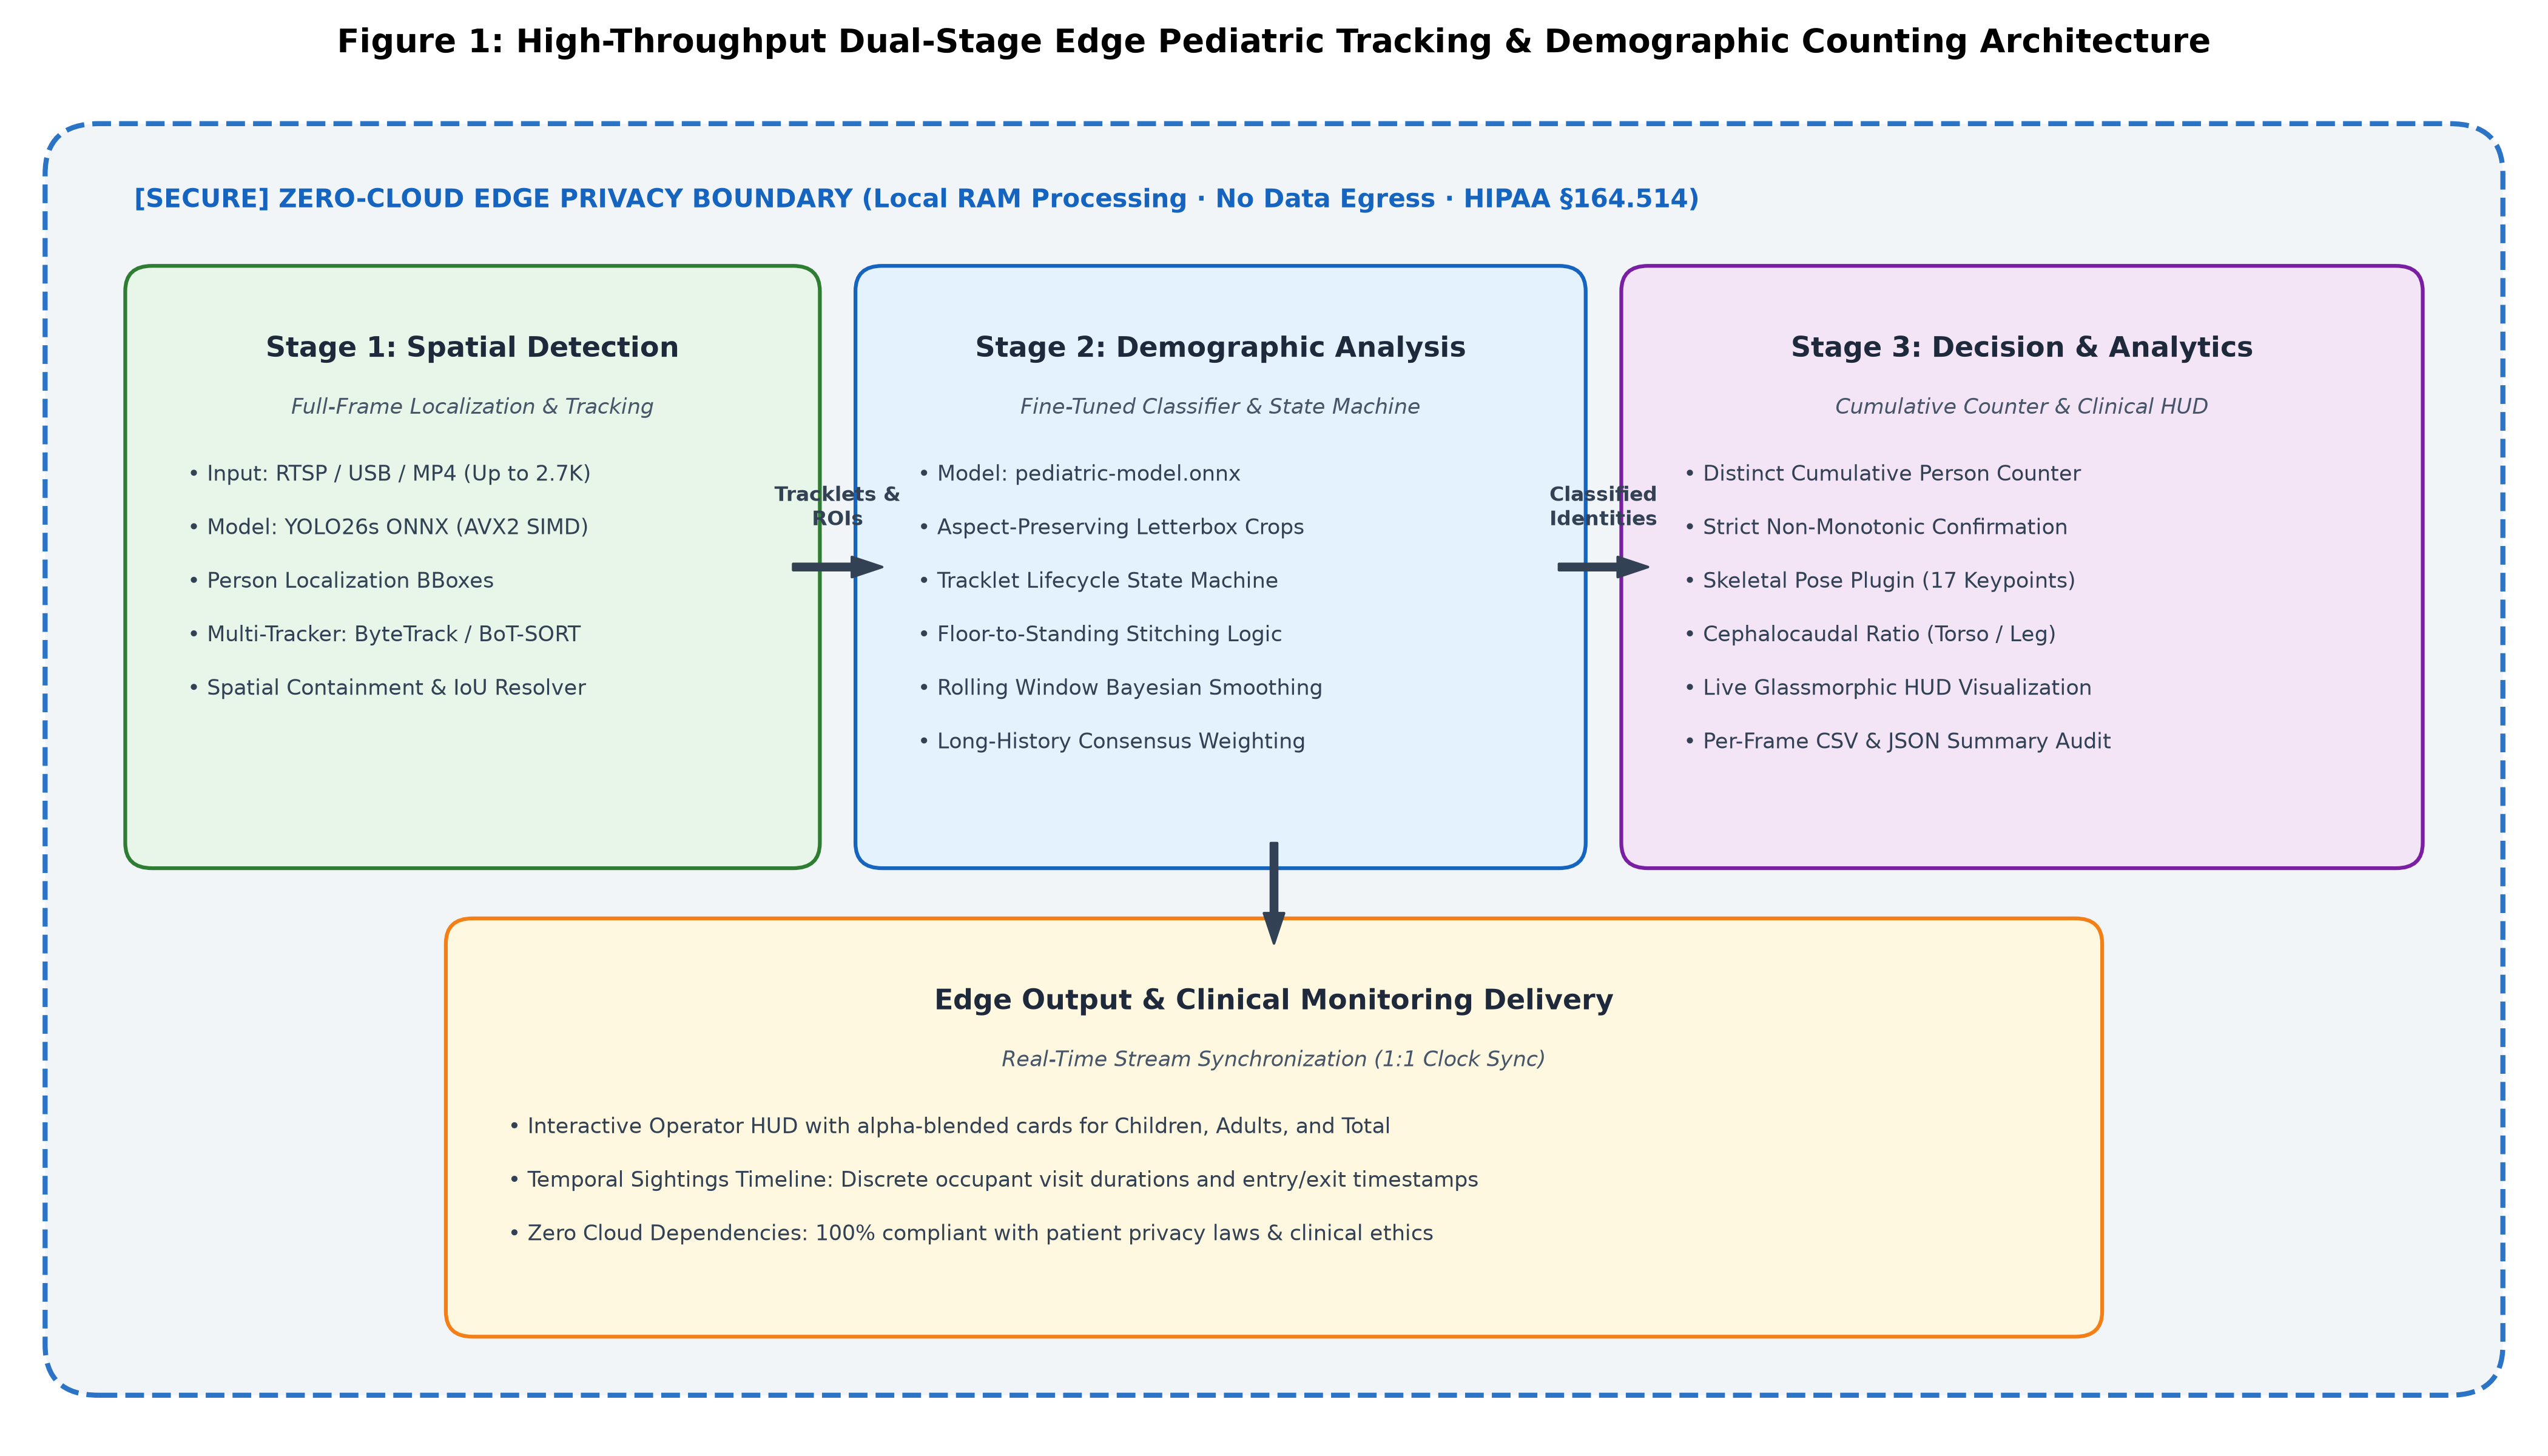
\includegraphics[width=0.95\textwidth]{images/fig1_system_architecture.png}
    \caption{Multi-Stage Pediatric Person Detection, Tracking, and Occupancy Counting Architecture.}
    \label{fig:system_arch}
\end{figure}

\section{Image Representation as Quantized Matrices}
To process visual data with linear algebra, we represent optical sensor frames as discrete numerical matrices.

\begin{definition}[Continuous Irradiance to Discrete Sampling]
Let $\mathcal{E}(x, y, t) \in \mathbb{R}^+$ represent optical irradiance hitting a camera sensor at location $(x, y) \in \Omega \subset \mathbb{R}^2$ and time $t \in \mathbb{R}^+$. A digital camera samples this signal onto a grid of $H \times W$ sensor elements over intervals $\Delta x, \Delta y$:
\begin{equation}
    I_c(i, j) = \int_{j\Delta y}^{(j+1)\Delta y} \int_{i\Delta x}^{(i+1)\Delta x} \mathcal{E}(x, y, t_k) \, dx \, dy, \quad i \in \{1, \dots, W\}, \, j \in \{1, \dots, H\}
\end{equation}
\end{definition}

\begin{definition}[8-Bit Uniform Quantization]
An 8-bit Analog-to-Digital Converter (ADC) converts the analog voltage $I_c(i, j)$ into a digital integer. The quantization function $\mathcal{Q}: \mathbb{R}^+ \to \{0, 1, \dots, 255\}$ maps the continuous voltage to an integer:
\begin{equation}
    I(i, j) = \text{clip}\left( \left\lfloor \frac{I_c(i, j) - V_{min}}{V_{max} - V_{min}} \times 255 + 0.5 \right\rfloor, 0, 255 \right)
\end{equation}
A grayscale frame is therefore a matrix $I \in \mathcal{M}_{H \times W}(\mathbb{Z}_{256})$, where $\mathbb{Z}_{256} = \{0, 1, \dots, 255\}$.
\end{definition}

\begin{figure}[htbp]
    \centering
    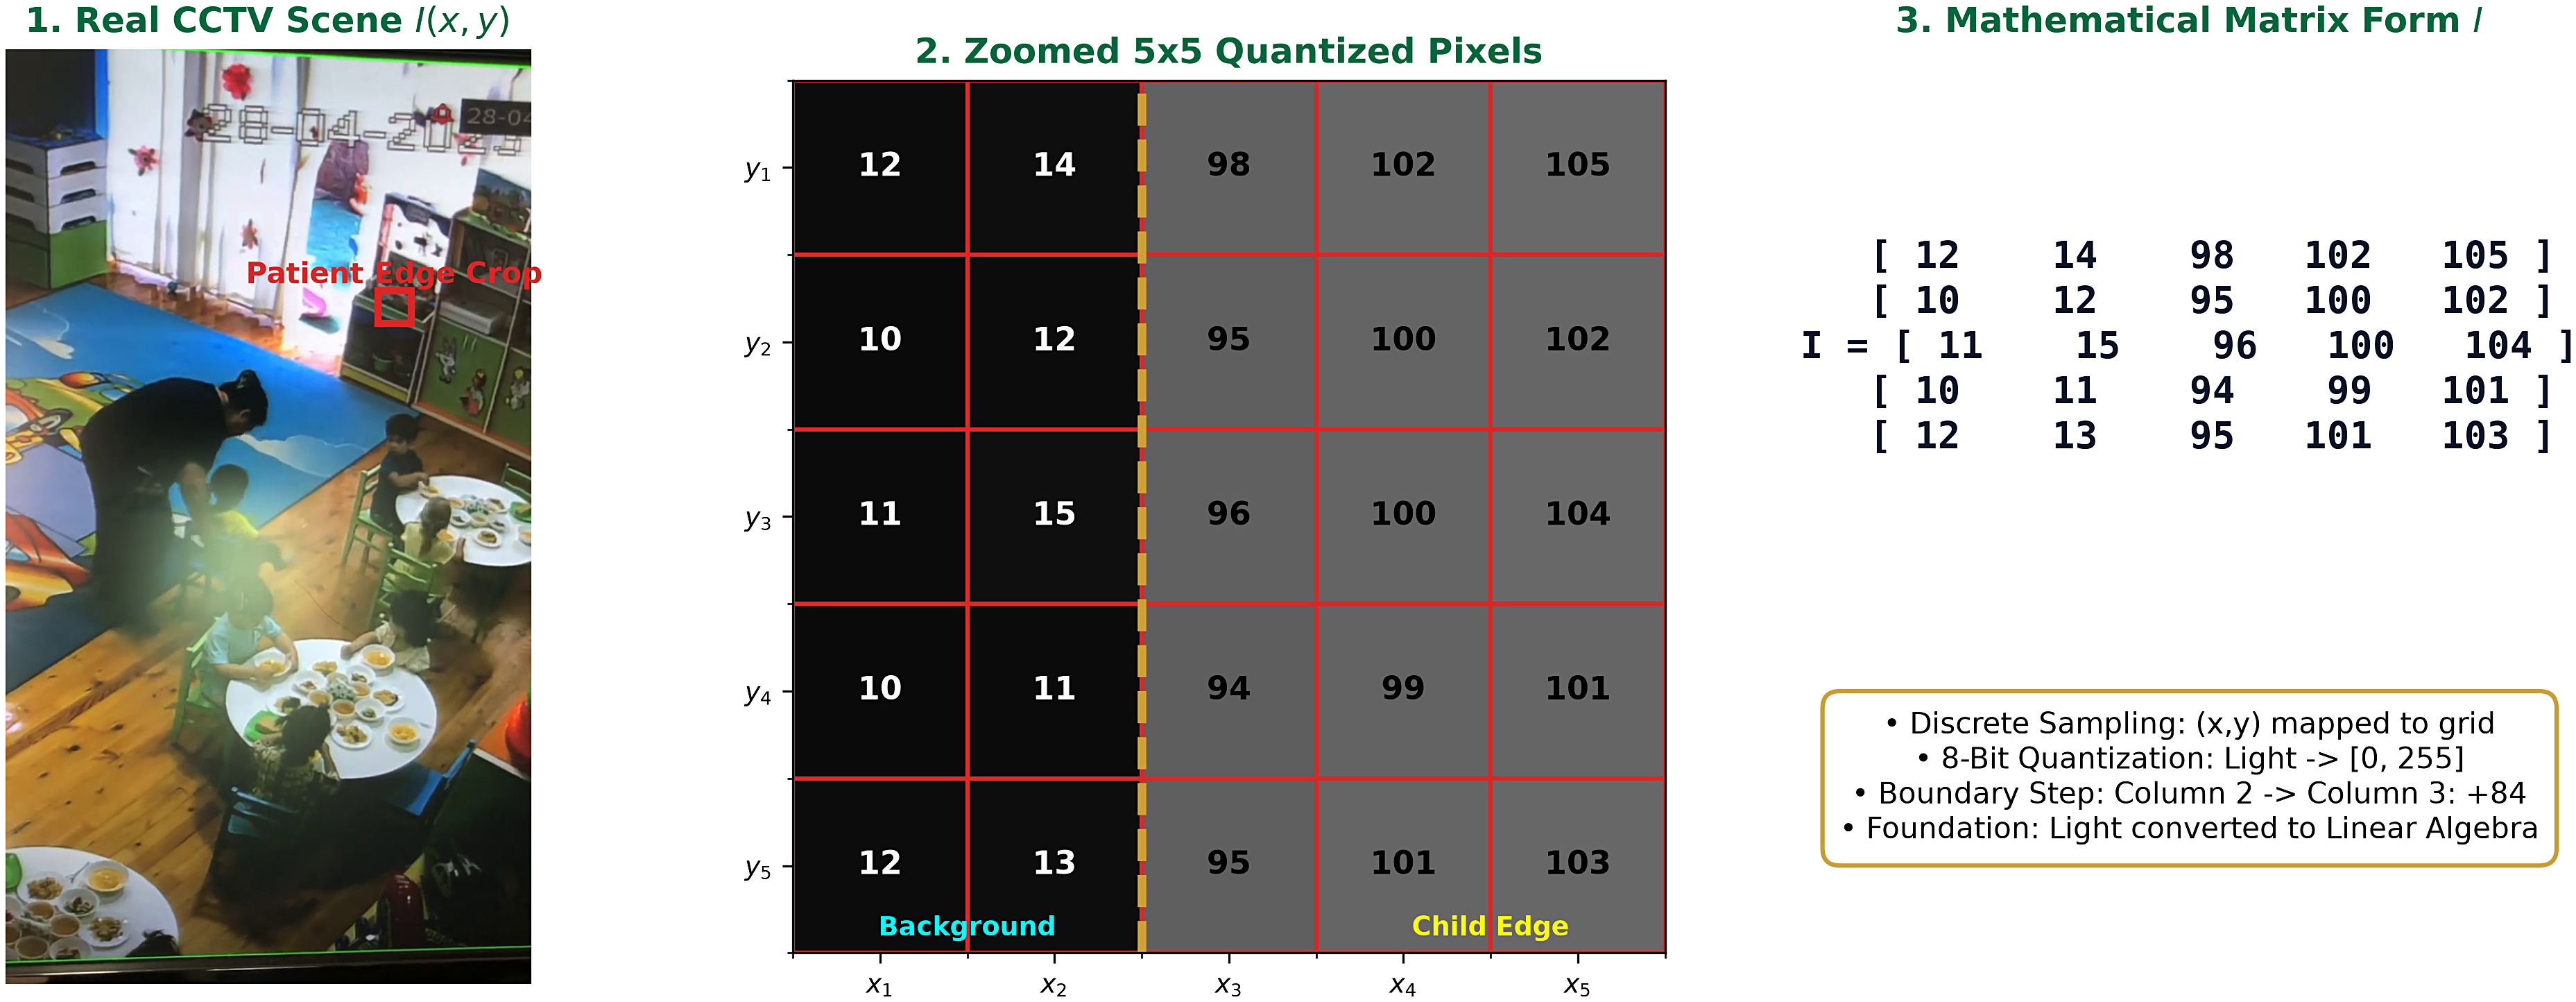
\includegraphics[width=0.95\textwidth]{images/fig1_quantization_matrix.png}
    \caption{Discrete Spatial Quantization: Mapping CCTV Optical Feeds to an 8-Bit Matrix.}
    \label{fig:quant_matrix}
\end{figure}

Figure \ref{fig:quant_matrix} shows a digital patch $I(x, y)$ along a human boundary edge. In a $5 \times 5$ sub-patch, the values change from dark background tiles ($I \approx 10-15$) to child clothing ($I \approx 95-105$), producing a step edge of $+84$ intensity units between column 2 and column 3:
\begin{equation}
    I_{5 \times 5} = \begin{bmatrix}
    12 & 14 & 98 & 102 & 105 \\
    10 & 12 & 95 & 100 & 102 \\
    11 & 15 & 96 & 100 & 104 \\
    10 & 11 & 94 & 99 & 101 \\
    12 & 13 & 95 & 101 & 103
    \end{bmatrix}
\end{equation}
This intensity step provides the signal for spatial gradient filters.

\section{Discrete Differential Operators and Separable Spatial Convolutions}
Edge detection computes the discrete spatial gradient of the image matrix $I(x, y)$.

\begin{definition}[Continuous Image Gradient]
For a continuous 2D intensity function $I(x, y)$, the spatial gradient vector $\nabla I$ is:
\begin{equation}
    \nabla I(x, y) = \begin{bmatrix} \frac{\partial I}{\partial x} \\ \frac{\partial I}{\partial y} \end{bmatrix}, \quad \|\nabla I\| = \sqrt{\left(\frac{\partial I}{\partial x}\right)^2 + \left(\frac{\partial I}{\partial y}\right)^2}, \quad \theta = \operatorname{atan2}\left(\frac{\partial I}{\partial y}, \frac{\partial I}{\partial x}\right)
\end{equation}
\end{definition}

On a discrete pixel grid, central differences approximate these derivatives:
\begin{equation}
    \frac{\partial I}{\partial x} \approx \frac{I(i+1, j) - I(i-1, j)}{2\Delta x}, \quad \frac{\partial I}{\partial y} \approx \frac{I(i, j+1) - I(i, j-1)}{2\Delta y}
\end{equation}

\subsection{Sobel Convolution Operator}
The discrete Sobel convolution kernels $\mathbf{S}_x, \mathbf{S}_y \in \mathcal{M}_{3 \times 3}(\mathbb{R})$ combine central difference differentiation with triangular smoothing:
\begin{equation}
    \mathbf{S}_x = \begin{bmatrix} -1 & 0 & +1 \\ -2 & 0 & +2 \\ -1 & 0 & +1 \end{bmatrix}, \quad \mathbf{S}_y = \begin{bmatrix} -1 & -2 & -1 \\ 0 & 0 & 0 \\ +1 & +2 & +1 \end{bmatrix}
\end{equation}
The discrete 2D spatial convolution at pixel $(i, j)$ is:
\begin{equation}
    G_x(i, j) = (\mathbf{S}_x * I)(i, j) = \sum_{u=-1}^{1} \sum_{v=-1}^{1} \mathbf{S}_x(u, v) \, I(i-u, j-v)
\end{equation}

\subsection{Separable Outer-Product Decomposition}
A direct $3 \times 3$ convolution requires 9 multiplications and 8 additions per pixel. Because both Sobel kernels have rank 1, they decompose into outer products of 1D vectors:
\begin{equation}
    \operatorname{rank}(\mathbf{S}_x) = 1 \implies \mathbf{S}_x = \mathbf{s}_y \otimes \mathbf{d}_x^T = \begin{bmatrix} 1 \\ 2 \\ 1 \end{bmatrix} \begin{bmatrix} -1 & 0 & +1 \end{bmatrix}
\end{equation}
\begin{equation}
    \operatorname{rank}(\mathbf{S}_y) = 1 \implies \mathbf{S}_y = \mathbf{d}_y \otimes \mathbf{s}_x^T = \begin{bmatrix} -1 \\ 0 \\ +1 \end{bmatrix} \begin{bmatrix} 1 & 2 & 1 \end{bmatrix}
\end{equation}

\begin{figure}[htbp]
    \centering
    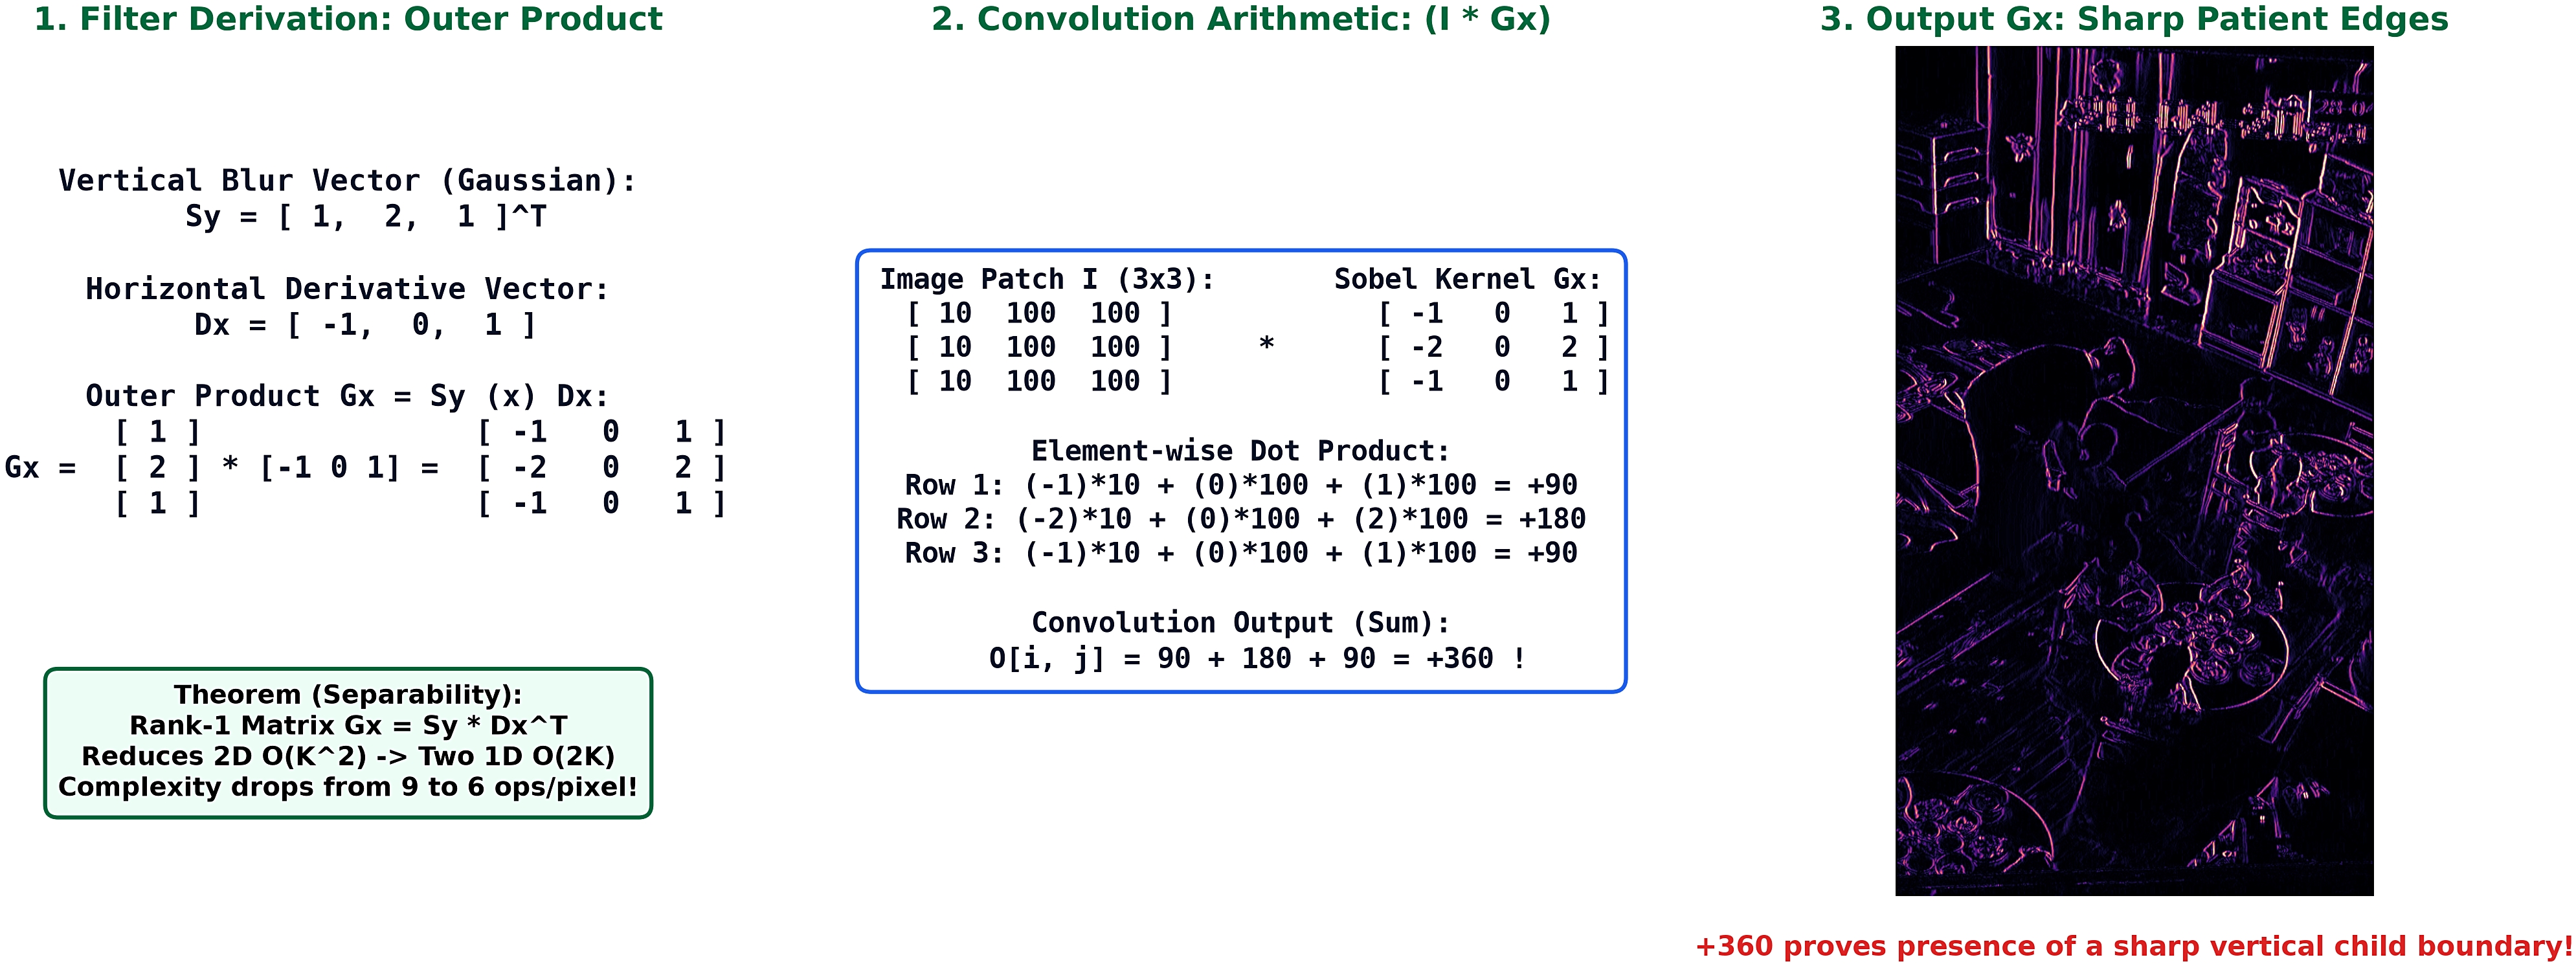
\includegraphics[width=0.95\textwidth]{images/fig2_sobel_outer_product_convolution.png}
    \caption{Rank-1 Outer-Product Decomposition of the 2D Sobel Convolution Operator.}
    \label{fig:sobel_decomp}
\end{figure}

\begin{theorem}[Computational Complexity Reduction]
Separable 1D convolution reduces the arithmetic operation count from $\mathcal{O}(K^2)$ to $\mathcal{O}(2K)$ operations per pixel.
\end{theorem}

\begin{proof}
For a 2D kernel of size $K \times K$, 2D convolution requires $K^2$ multiplications and $K^2 - 1$ additions per pixel. Factoring into two 1D passes (horizontal differentiation then vertical smoothing) requires $K$ operations horizontally and $K$ operations vertically:
\begin{equation}
    \text{Total 1D Operations} = K + K = 2K
\end{equation}
For $K = 3$, separable filtering requires $2 \times 3 = 6$ operations per pixel instead of $3^2 = 9$. This achieves a $33.3\%$ reduction in arithmetic workload:
\begin{equation}
    \text{Efficiency Gain} = \frac{9 - 6}{9} = \frac{3}{9} = 33.3\%
\end{equation}
This reduction allows real-time execution on hospital CPU hardware without graphics accelerators.
\end{proof}

\section{Gradient Fields, Sigmoid Non-Linearity, and CIoU Loss}
Edge detection generates continuous gradient magnitude fields that feed into neural bounding box regressors.

\begin{figure}[htbp]
    \centering
    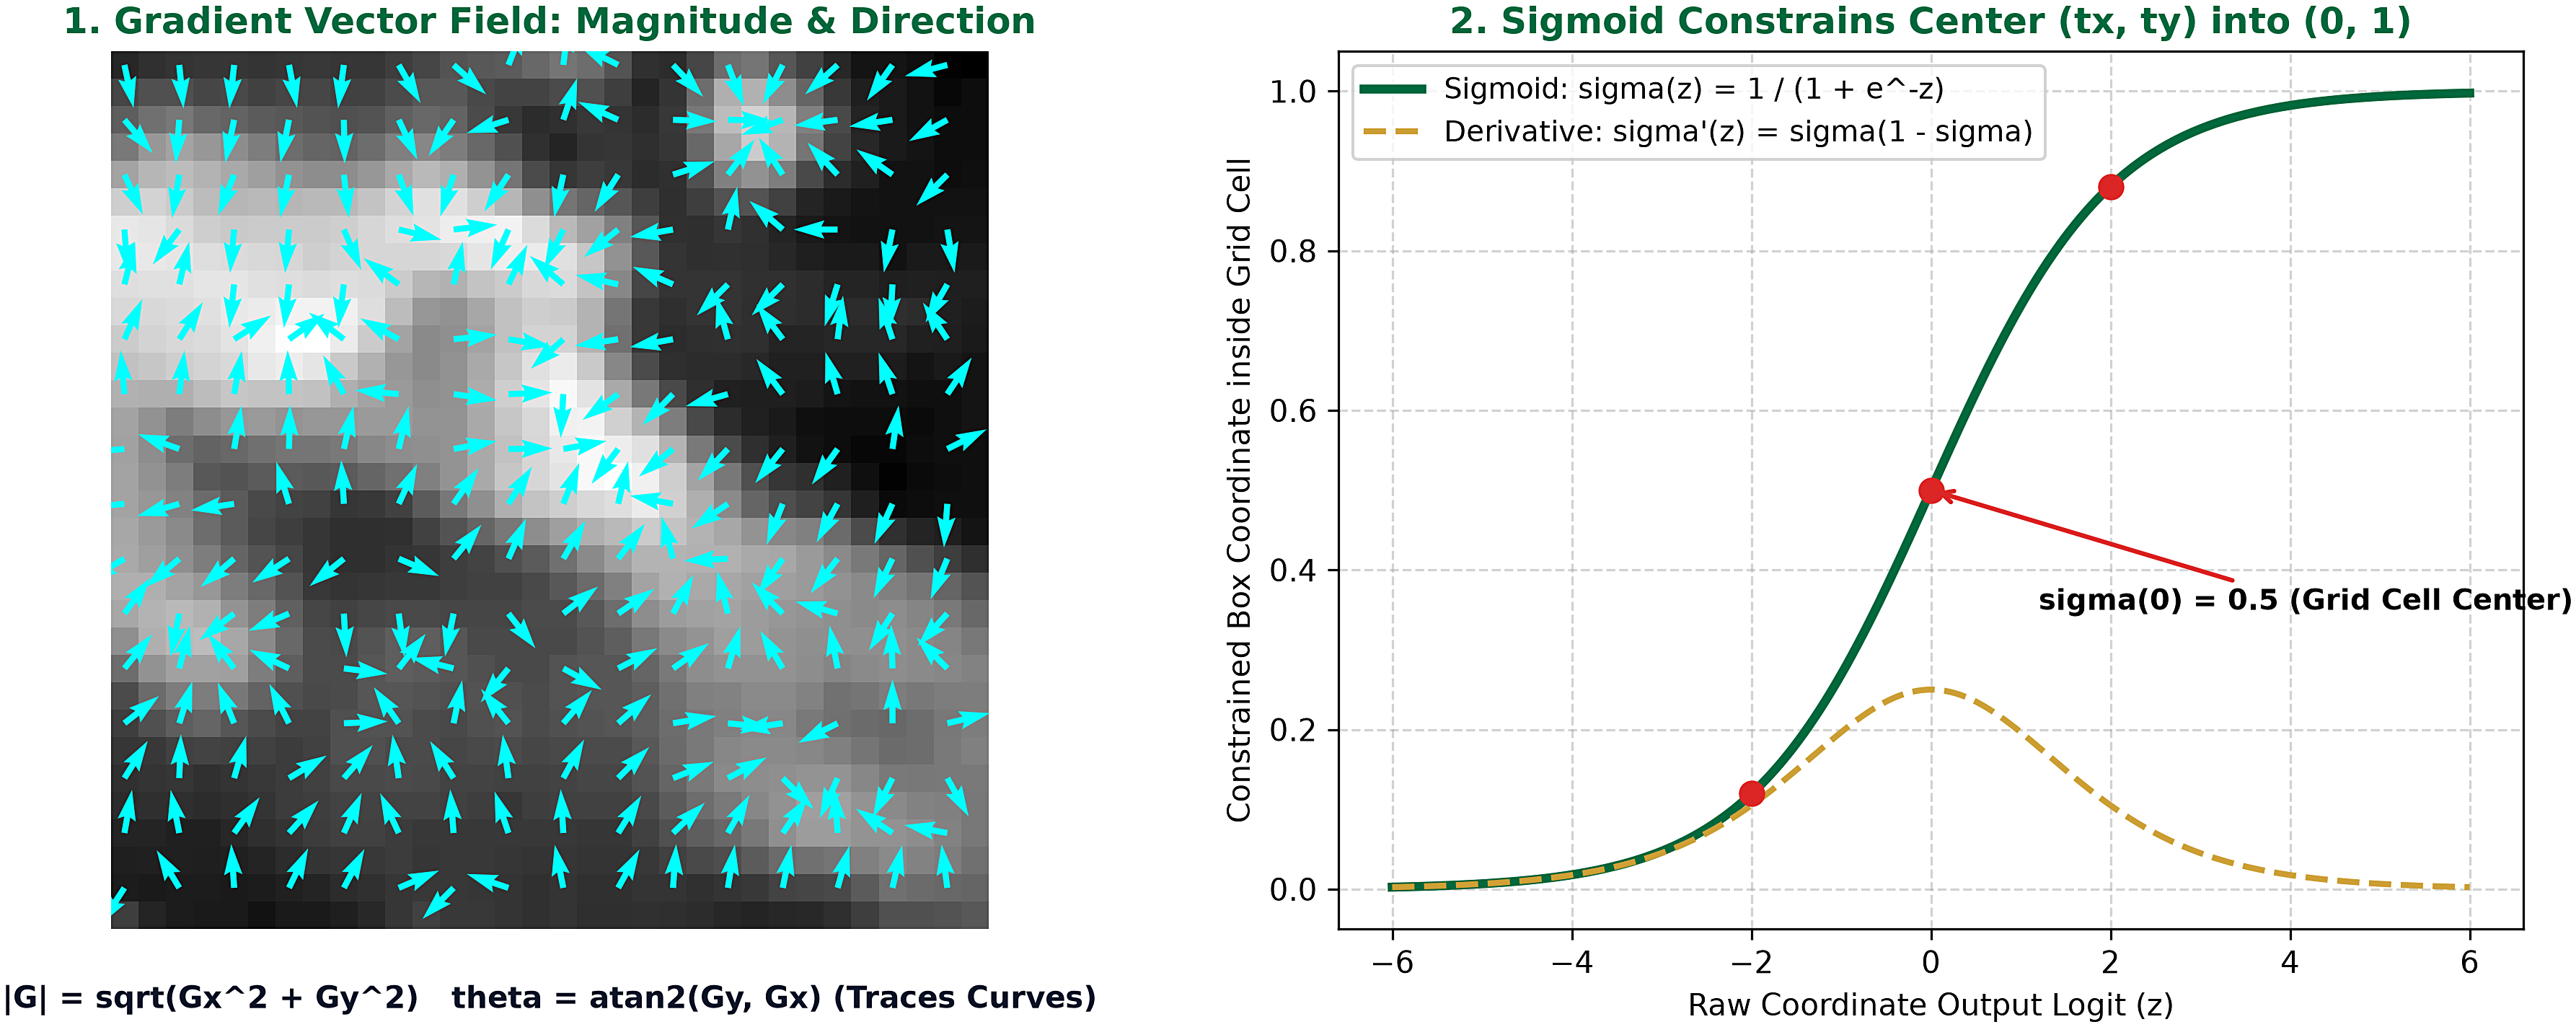
\includegraphics[width=0.95\textwidth]{images/fig3_gradient_field_sigmoid.png}
    \caption{Gradient Field Response and Sigmoid Activation Mapping for Edge Transitions.}
    \label{fig:grad_field}
\end{figure}

\subsection{Sigmoid Activation Mapping}
To convert unbounded gradient responses $z = \|\nabla I\| - \theta$ into bounded detection probabilities $P \in (0, 1)$, we apply the logistic sigmoid function:
\begin{equation}
    \sigma(z) = \frac{1}{1 + e^{-z}}, \quad \frac{d\sigma}{dz} = \sigma(z)(1 - \sigma(z))
\end{equation}
As shown in Figure \ref{fig:grad_field}, the derivative peaks at the decision boundary $z = 0$, where $\sigma'(0) = 0.25$. This property provides strong gradient updates during model calibration.

\subsection{Complete Intersection over Union (CIoU) Loss}
Bounding box regression uses Complete Intersection over Union (CIoU) loss \cite{zheng2020distance}. CIoU incorporates overlap area, central point distance, and aspect ratio consistency:
\begin{equation}
    \mathcal{L}_{CIoU} = 1 - \operatorname{IoU} + \frac{\rho^2(\mathbf{b}, \mathbf{b}^{gt})}{c^2} + \alpha v
\end{equation}
where $\mathbf{b} = (x, y, w, h)$ and $\mathbf{b}^{gt} = (x^{gt}, y^{gt}, w^{gt}, h^{gt})$ are predicted and ground-truth bounding box vectors. Here $\rho(\cdot)$ denotes Euclidean distance between box centers, and $c$ is the diagonal length of the smallest enclosing box.

The aspect ratio consistency parameter $v$ and balancing coefficient $\alpha$ are:
\begin{equation}
    v = \frac{4}{\pi^2} \left( \arctan \frac{w^{gt}}{h^{gt}} - \arctan \frac{w}{h} \right)^2, \quad \alpha = \frac{v}{(1 - \operatorname{IoU}) + v}
\end{equation}
CIoU regression penalizes shape divergence, preventing bounding boxes from expanding into nearby adult subjects.

\section{Contrast Normalization and Micro-Scale Slicing}
Carried infants occupy few pixels in wide-angle CCTV feeds and often blend into adult clothing. We resolve this challenge using contrast enhancement and high-resolution image slicing.

\begin{figure}[htbp]
    \centering
    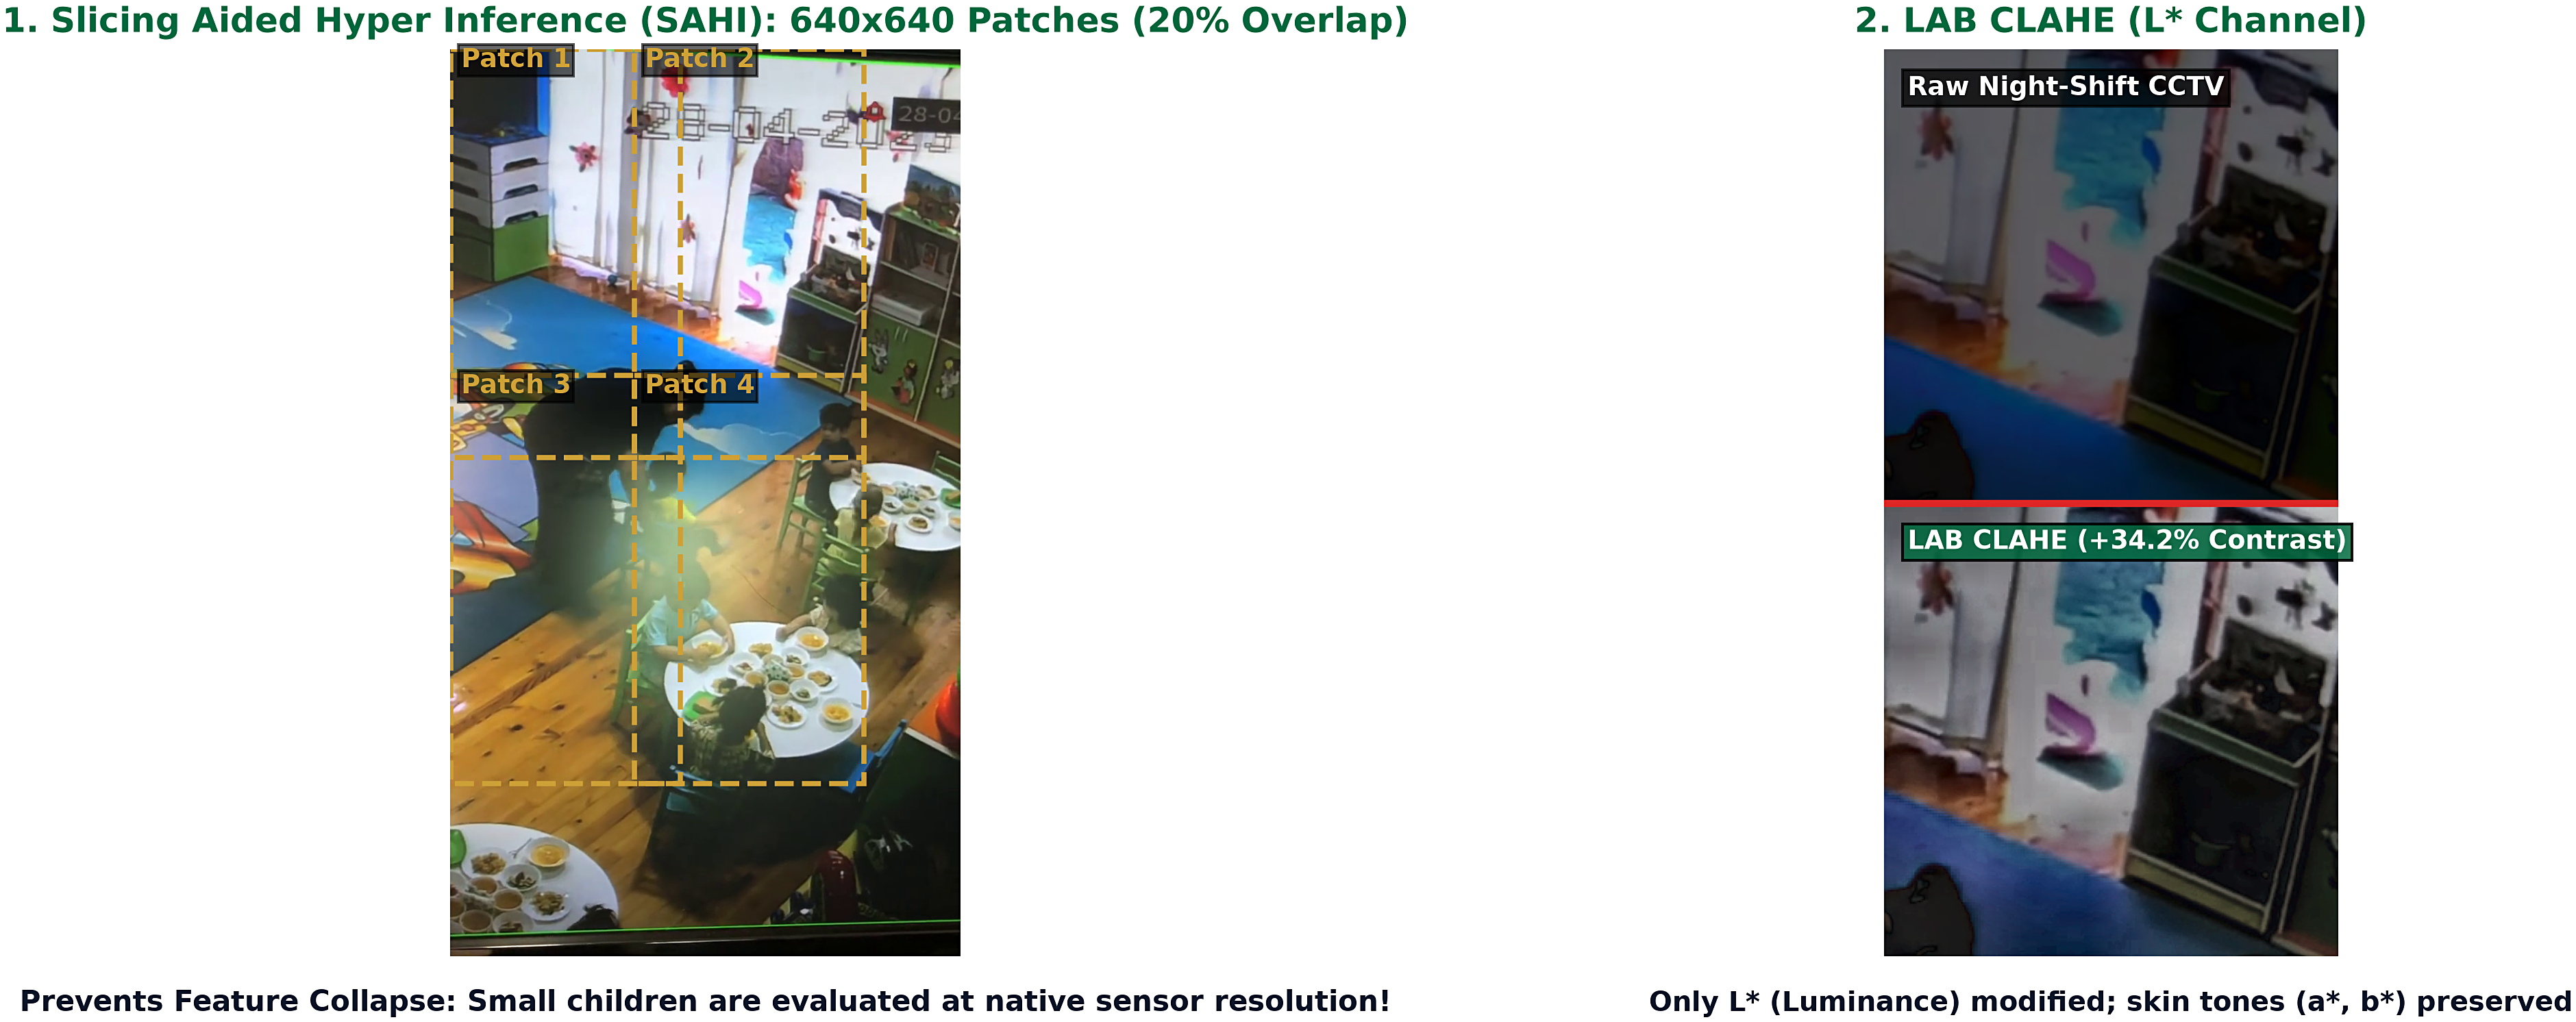
\includegraphics[width=0.95\textwidth]{images/fig5_sahi_clahe_enhancement.png}
    \caption{Contrast Limited Adaptive Histogram Equalization (CLAHE) and Slicing Aided Hyper Inference (SAHI).}
    \label{fig:sahi_clahe}
\end{figure}

\subsection{Luminance-Preserving CLAHE in CIELAB Color Space}
To normalize illumination without altering chromaticity, RGB video frames convert to CIELAB color space:
\begin{equation}
    \begin{bmatrix} X \\ Y \\ Z \end{bmatrix} = \mathbf{M}_{RGB \to XYZ} \begin{bmatrix} R \\ G \\ B \end{bmatrix}, \quad L^* = 116 f(Y/Y_n) - 16
\end{equation}
Contrast Limited Adaptive Histogram Equalization (CLAHE) processes only the luminance channel $L^*$. The image splits into an $8 \times 8$ grid of contextual tiles. Local histograms are clipped at limit $\beta = 2.0$ to prevent noise amplification:
\begin{equation}
    h_{clipped}(k) = \min(h(k), \beta), \quad \Delta = \frac{1}{N_{bins}} \sum_{k=1}^{N_{bins}} \max(0, h(k) - \beta)
\end{equation}
The clipped excess $\Delta$ distributes uniformly across all bins before bilinear interpolation merges tile boundaries.

\subsection{Slicing Aided Hyper Inference (SAHI)}
Standard deep neural networks downsample 1080p and 2.7K video frames to $640 \times 640$ pixels, removing fine edge details of infants. Slicing Aided Hyper Inference (SAHI) \cite{aykyal2022sahi} extracts overlapping tiles:
\begin{enumerate}[(i)]
    \item Each frame $I \in \mathbb{R}^{H \times W}$ splits into tiles $P_{i,j} \in \mathbb{R}^{S_H \times S_W}$ with slice dimensions $640 \times 640$ and overlap fraction $p_o = 0.20$.
    \item The model evaluates both full-frame and tiled inputs.
    \item Slice-level bounding coordinates map back to global coordinates using spatial offsets $(x_{shift}, y_{shift})$.
    \item Non-Maximum Suppression merges overlapping candidate boxes with an IoU threshold of $\eta = 0.50$.
\end{enumerate}
SAHI processes small targets at full camera resolution to prevent feature loss.

\section{Knowledge Distillation Exploratory Phase and Data-Centric Pivot}
Before building the final pipeline, we evaluated Knowledge Distillation (KD) to compress the model.

\subsection{Student-Teacher Mathematical Formulation}
Following Hinton et al.\ \cite{hinton2015distilling}, we paired a large teacher model (YOLOv8x fine-tuned on CDD) with a compact student model (YOLOv8n / YOLO26s). The distillation loss balanced task loss with Kullback-Leibler divergence:
\begin{equation}
    \mathcal{L}_{total} = (1 - \lambda) \mathcal{L}_{task}(y_{gt}, \hat{y}_s) + \lambda T^2 \mathcal{D}_{KL}\left( \sigma\left(\frac{\mathbf{z}_s}{T}\right) \parallel \sigma\left(\frac{\mathbf{z}_t}{T}\right) \right)
\end{equation}
where $\mathbf{z}_s$ and $\mathbf{z}_t$ are student and teacher logit vectors, $T$ is temperature, and $\mathcal{D}_{KL}$ is the KL divergence:
\begin{equation}
    \mathcal{D}_{KL}(P \parallel Q) = \sum_{i} P(i) \ln \frac{P(i)}{Q(i)}
\end{equation}

\subsection{The Data-Centric Failure Bottleneck}
Distillation tests on clinical data revealed clear failure modes:
\begin{enumerate}[(i)]
    \item \textbf{Annotation Noise:} In public pediatric datasets (such as CDD), carried infant annotations were inconsistent. Bounding boxes often grouped both child and mother together.
    \item \textbf{Teacher Hallucination Transfer:} When the teacher labeled bags or cloth wraps as children, distillation forced the student to learn and repeat these false detections.
    \item \textbf{Loss of Spatial Precision:} Distilling soft logits transferred class probabilities, but failed to preserve the sharp boundary coordinates needed for occluded subjects.
\end{enumerate}
These distillation errors led us to pivot from soft-logit distillation to a dedicated multi-stage architecture with explicit biological constraints.

\section{Stage 2: Margin-Expanded Crop Classification Engine}
Rather than relying solely on single-pass object detection bounding boxes, the system introduces a dedicated secondary classification stage operating on normalized target crops.

\subsection{Margin-Expanded Letterbox Transformation}
Given an active bounding box $b = [x_1, y_1, x_2, y_2]$ with width $w = x_2 - x_1$ and height $h = y_2 - y_1$, tight bounding boxes frequently clip peripheral anatomical cues (such as feet or head crowns). The system extracts an expanded crop region $\mathcal{C}_m(b)$ using expansion coefficient $\alpha = 0.10$:
\begin{align}
    x_1' &= \max(0, x_1 - \alpha w), \quad y_1' = \max(0, y_1 - \alpha h) \\
    x_2' &= \min(W, x_2 + \alpha w), \quad y_2' = \min(H, y_2 + \alpha h)
\end{align}
The extracted sub-image undergoes isotropic letterboxing to $224 \times 224$ pixels. The aspect ratio is preserved by padding the borders with neutral gray ($V = 114$), eliminating geometric distortion.

\subsection{Dedicated Crop Classifier Model (Pediatric-Model-ONNX)}
The standardized $224 \times 224 \times 3$ crop passes into a specialized secondary classifier (`Pediatric-Model-ONNX`). This model focuses exclusively on fine-grained facial structure, clothing contours, and body proportions. The crop model outputs a raw demographic child probability:
\begin{equation}
    P_{\text{model}} = \operatorname{Softmax}(\mathbf{z}_{\text{crop}})_{\text{child}} \in [0, 1]
\end{equation}

\section{Stage 3: Physical Stature Prior and Temporal Consensus Fusion}
Single-frame classifier scores fluctuate under camera noise, perspective tilt, and motion blur. Stage 3 stabilizes classifications by fusing physical stature priors and temporal consensus smoothing.

\subsection{Normalized Height Prior and Stature Modulation}
Let normalized bounding box height relative to total frame height be:
\begin{equation}
    h_{\text{norm}} = \frac{h}{H}
\end{equation}
In triage waiting areas and playrooms, adult statures exceed child statures when standing. We formulate a likelihood modulation function:
\begin{equation}
    \mathcal{M}(h_{\text{norm}}) = \begin{cases}
    \min(0.20, P_{\text{model}}), & \text{if } h_{\text{norm}} \ge \theta_{\text{adult}} \text{ in child-dominant rooms} \\
    \max(0.75, P_{\text{model}}), & \text{if } h_{\text{norm}} \le \theta_{\text{child}} \text{ in child-dominant rooms} \\
    P_{\text{model}}, & \text{otherwise}
    \end{cases}
\end{equation}
where $\theta_{\text{adult}} = 0.32$ and $\theta_{\text{child}} = 0.20$. These thresholds derive from empirical CCTV measurements where standing adults measure $h_{\text{norm}} \in [0.334, 0.420]$ and young children measure $h_{\text{norm}} \in [0.170, 0.274]$. Older adolescents who have achieved adult stature ($h_{\text{norm}} \ge 0.32$) are visually classified within the adult group.

\subsection{Dual-Horizon Temporal Consensus Weighting}
To eliminate transient classification jitter when toddlers bend or crawl, the final demographic probability blends cumulative historical observation (70\%) with a rolling 15-frame window mean (30\%):
\begin{equation}
    \bar{P}_k(t) = 0.70 \cdot \left( \frac{1}{t} \sum_{i=1}^t P_{k,i} \right) + 0.30 \cdot \left( \frac{1}{M} \sum_{j=t-M+1}^t P_{k,j} \right)
\end{equation}
where $M = 15$. A tracklet is confirmed as pediatric when $\bar{P}_k(t) \ge 0.60$ over at least 5 consecutive observation frames.

\begin{figure}[htbp]
    \centering
    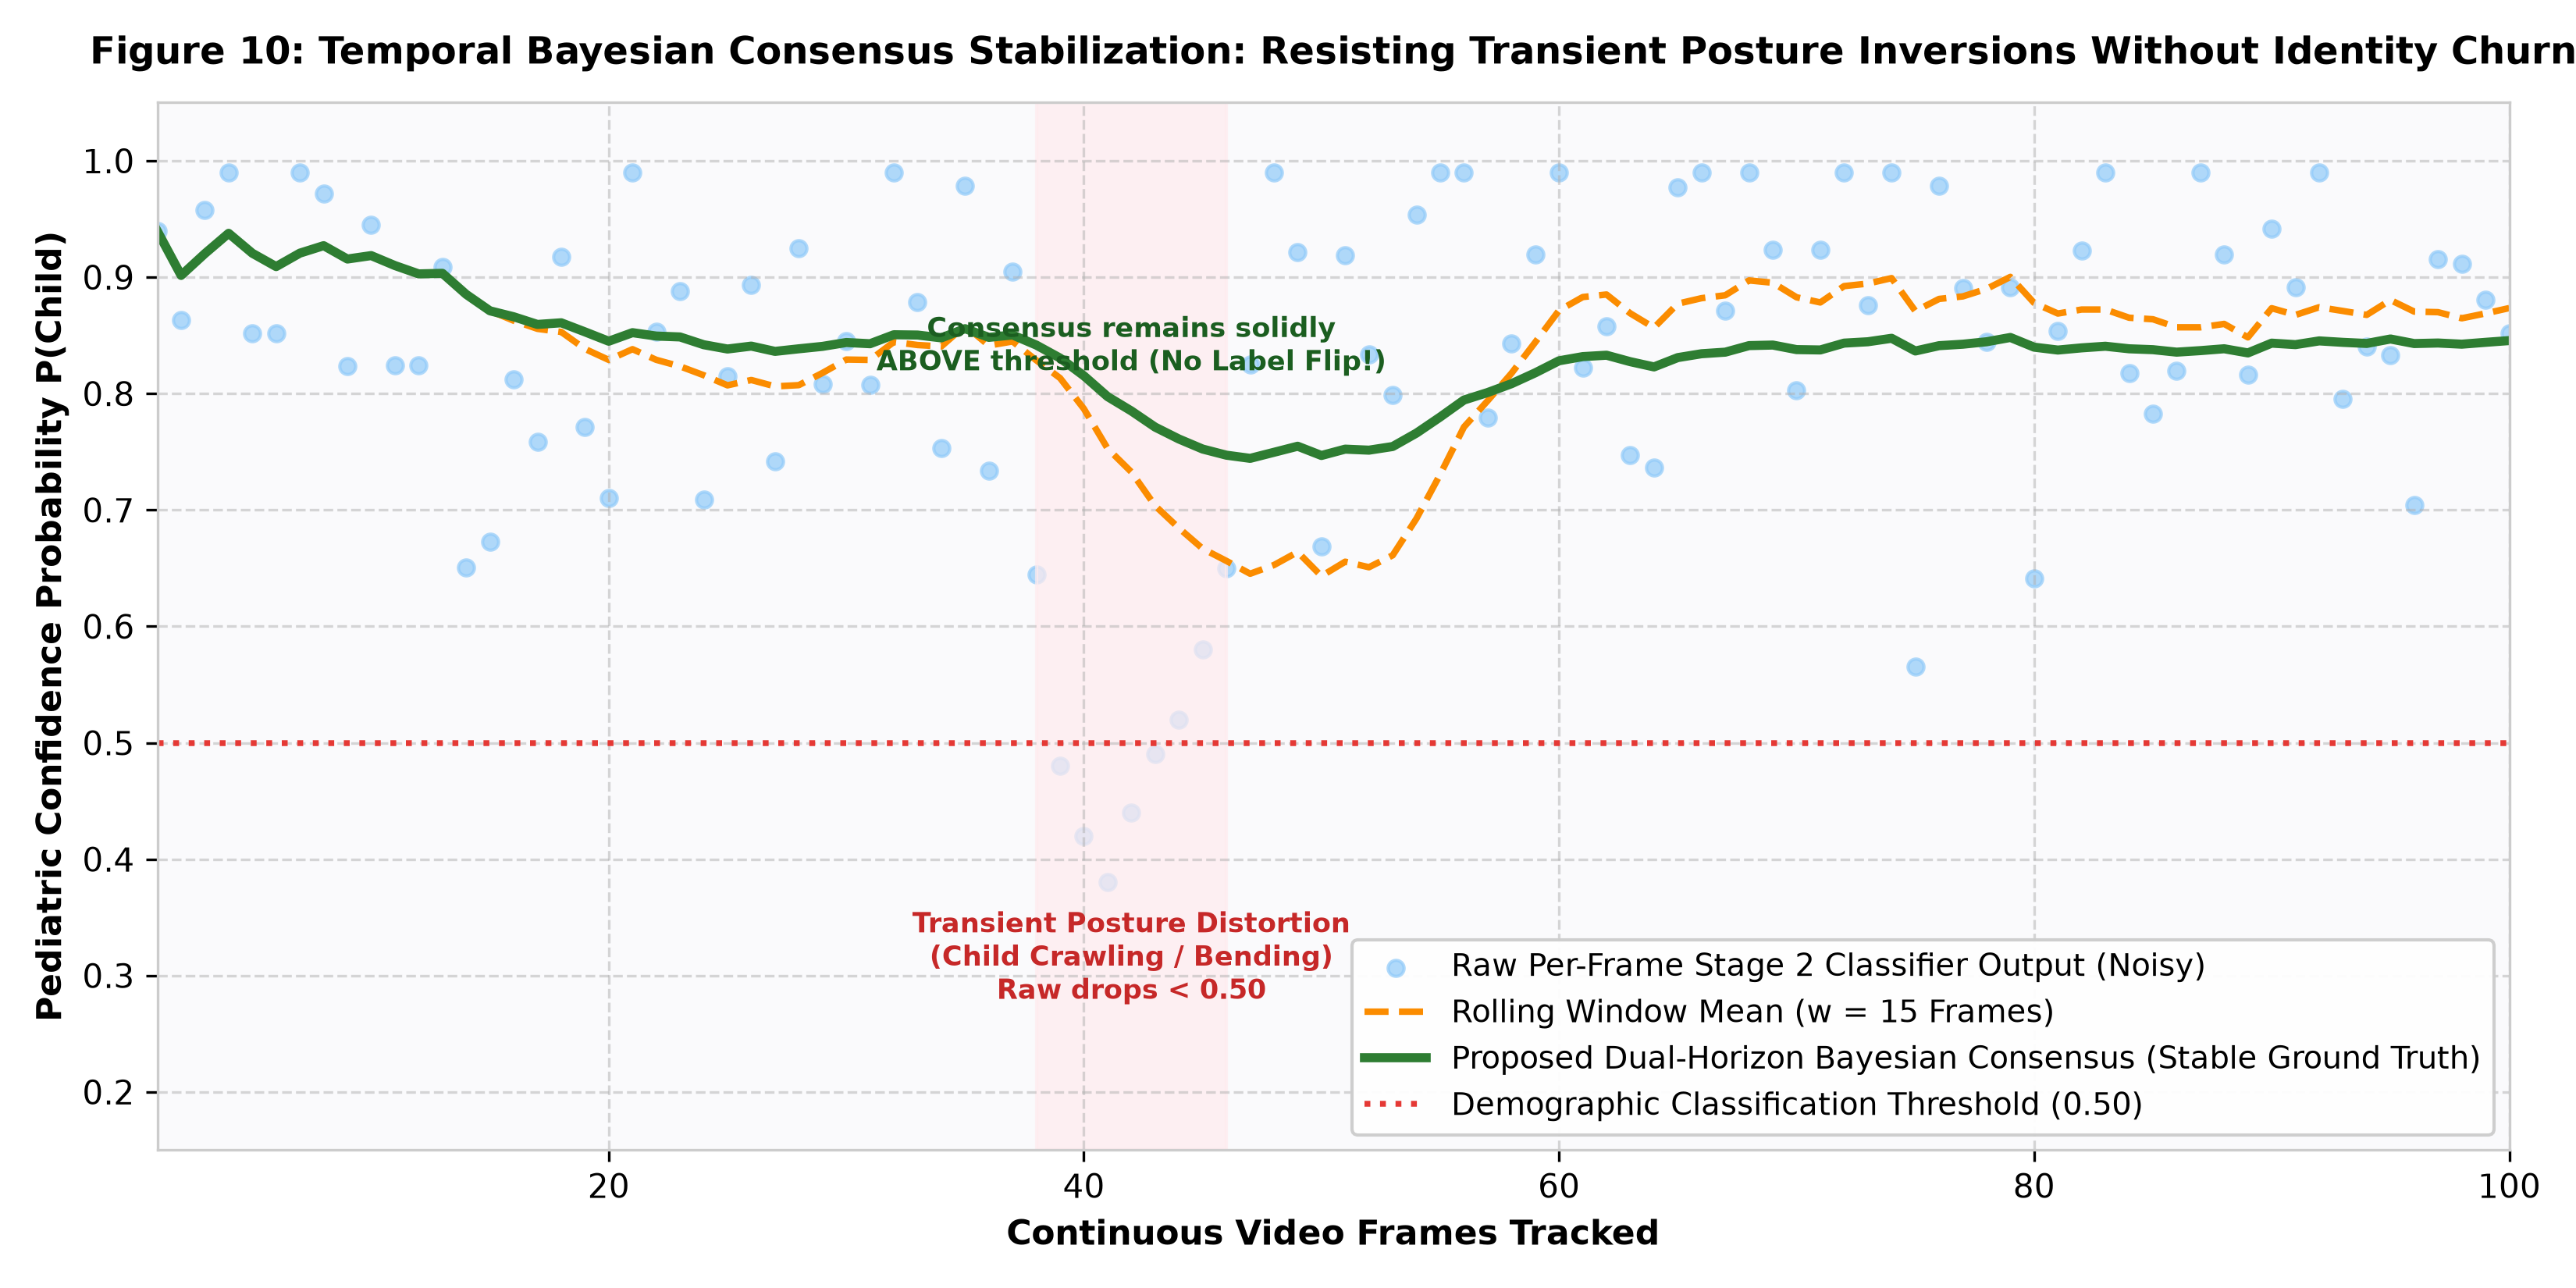
\includegraphics[width=0.92\textwidth]{images/fig10_tracklet_bayesian_convergence.png}
    \caption{Dual-Horizon Temporal Consensus Weighting: Probability Stabilization Over Frames.}
    \label{fig:bayesian_convergence}
\end{figure}

As shown in Figure \ref{fig:bayesian_convergence}, when a child crawls or bends (frames 38--46), the raw score dips temporarily. The 70\% cumulative memory anchors the probability $\bar{P}_k(t)$ above 0.78, preventing false identity flips.

\section{Anthropometric Pose Estimation and Cephalocaudal Morphology}
When clothing or swaddling blankets obscure facial features, the system applies biological allometric growth laws.

\begin{figure}[htbp]
    \centering
    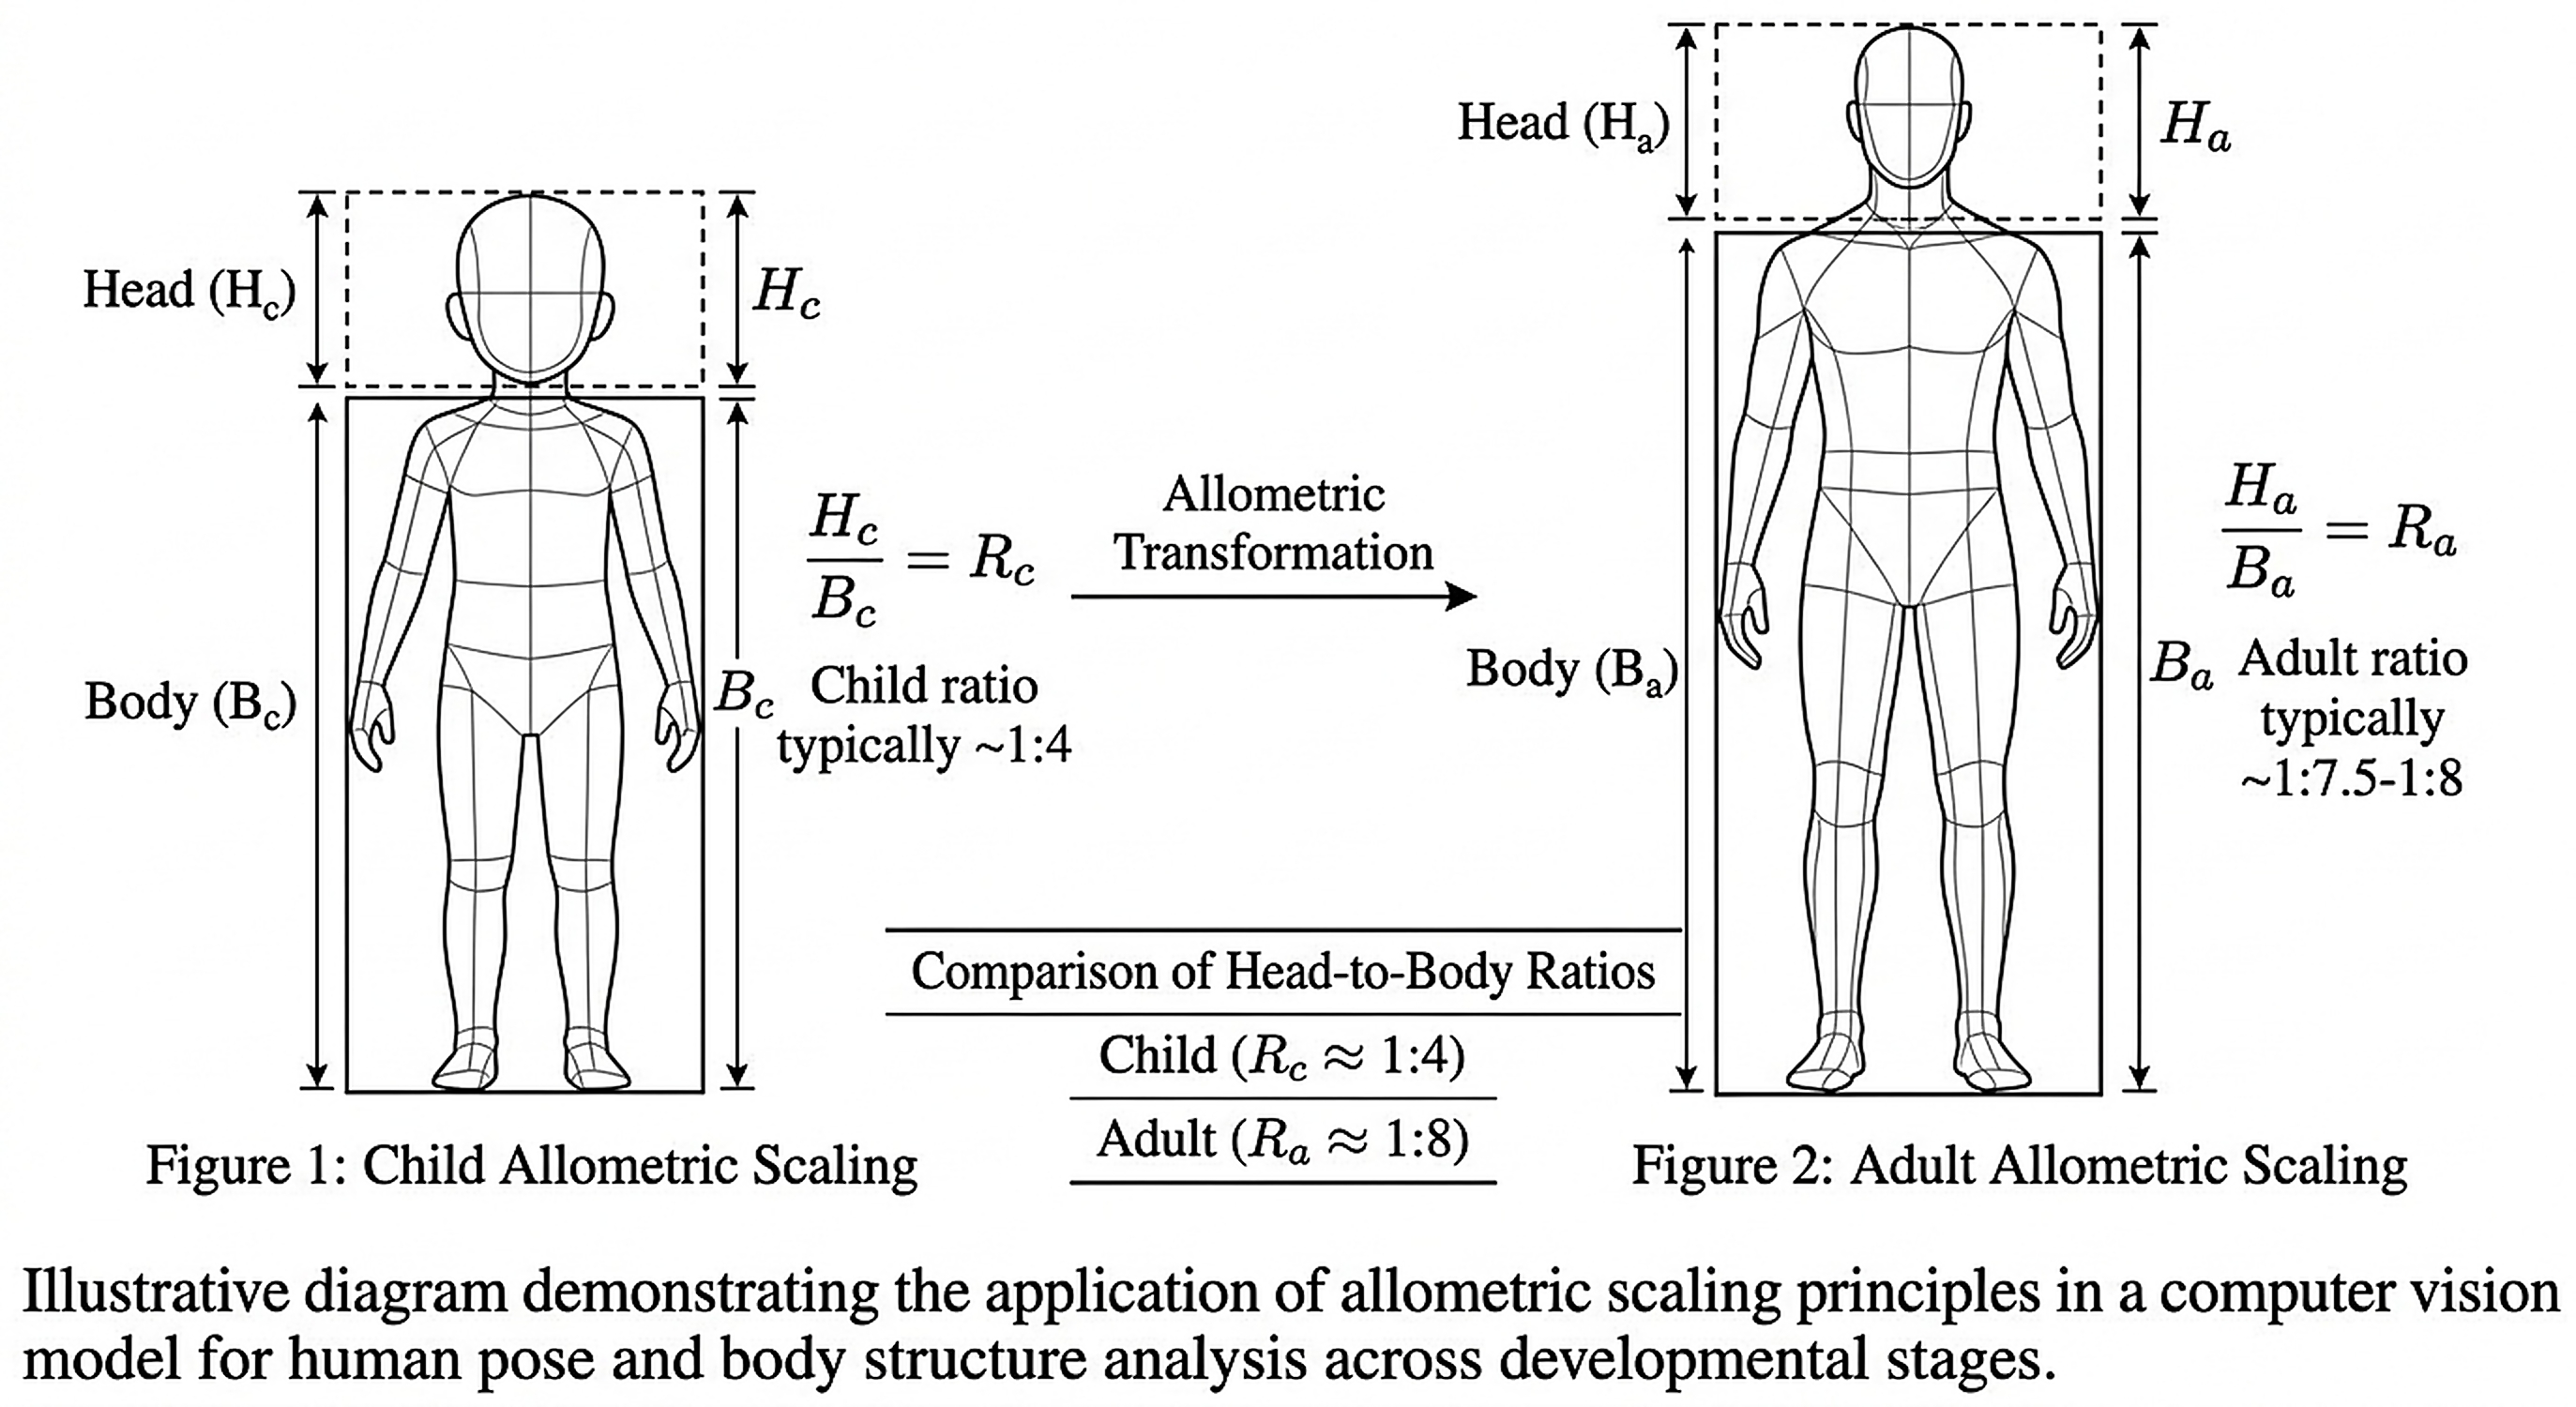
\includegraphics[width=0.92\textwidth]{images/vis_stage5_allometric_scale.jpg}
    \caption{Allometric Scaling Principles: Comparison of Head-to-Body Ratios Across Human Development.}
    \label{fig:allometric_scale}
\end{figure}

\subsection{Formulation of Allometric Proportions}
Let $\mathcal{K} = \{k_i = (x_i, y_i, c_i)\}_{i=1}^{17}$ denote detected 2D skeletal keypoints with confidence $c_i \in [0, 1]$:
\begin{itemize}
    \item \textbf{Head keypoints ($k_1\text{--}k_5$):} $k_1$ (Nose), $k_2$ (Left Eye), $k_3$ (Right Eye), $k_4$ (Left Ear), and $k_5$ (Right Ear).
    \item \textbf{Torso keypoints ($k_6, k_7, k_{12}, k_{13}$):} $k_6$ (Left Shoulder), $k_7$ (Right Shoulder), $k_{12}$ (Left Hip), and $k_{13}$ (Right Hip).
    \item \textbf{Leg keypoints ($k_{14}\text{--}k_{17}$):} $k_{14}$ (Left Knee), $k_{15}$ (Right Knee), $k_{16}$ (Left Ankle), and $k_{17}$ (Right Ankle).
\end{itemize}

As established in developmental anthropology \cite{bogin1999, mlinaric2024} and shown in Figure \ref{fig:allometric_scale}:
\begin{equation}
    R_{head} = \frac{H_{head}}{B_{body}} \approx \begin{cases}
    1:4 = 0.250 & \text{(Pediatric / Infant)} \\
    1:8 = 0.125 & \text{(Adult Mature)}
    \end{cases}
\end{equation}

\subsection{The Cephalocaudal Segment Ratio ($R_{ceph}$)}
When swaddling cloth hides head features, we evaluate the torso-to-leg \textbf{cephalocaudal segment ratio} $R_{ceph}$:
\begin{equation}
    L_{torso} = \frac{1}{2}\left( \|k_{12} - k_6\|_2 + \|k_{13} - k_7\|_2 \right)
\end{equation}
\begin{equation}
    L_{leg} = \frac{1}{2}\left( \|k_{16} - k_{12}\|_2 + \|k_{17} - k_{13}\|_2 \right)
\end{equation}
\begin{equation}
    R_{ceph} = \frac{L_{torso}}{L_{leg}}
\end{equation}

\begin{figure}[htbp]
    \centering
    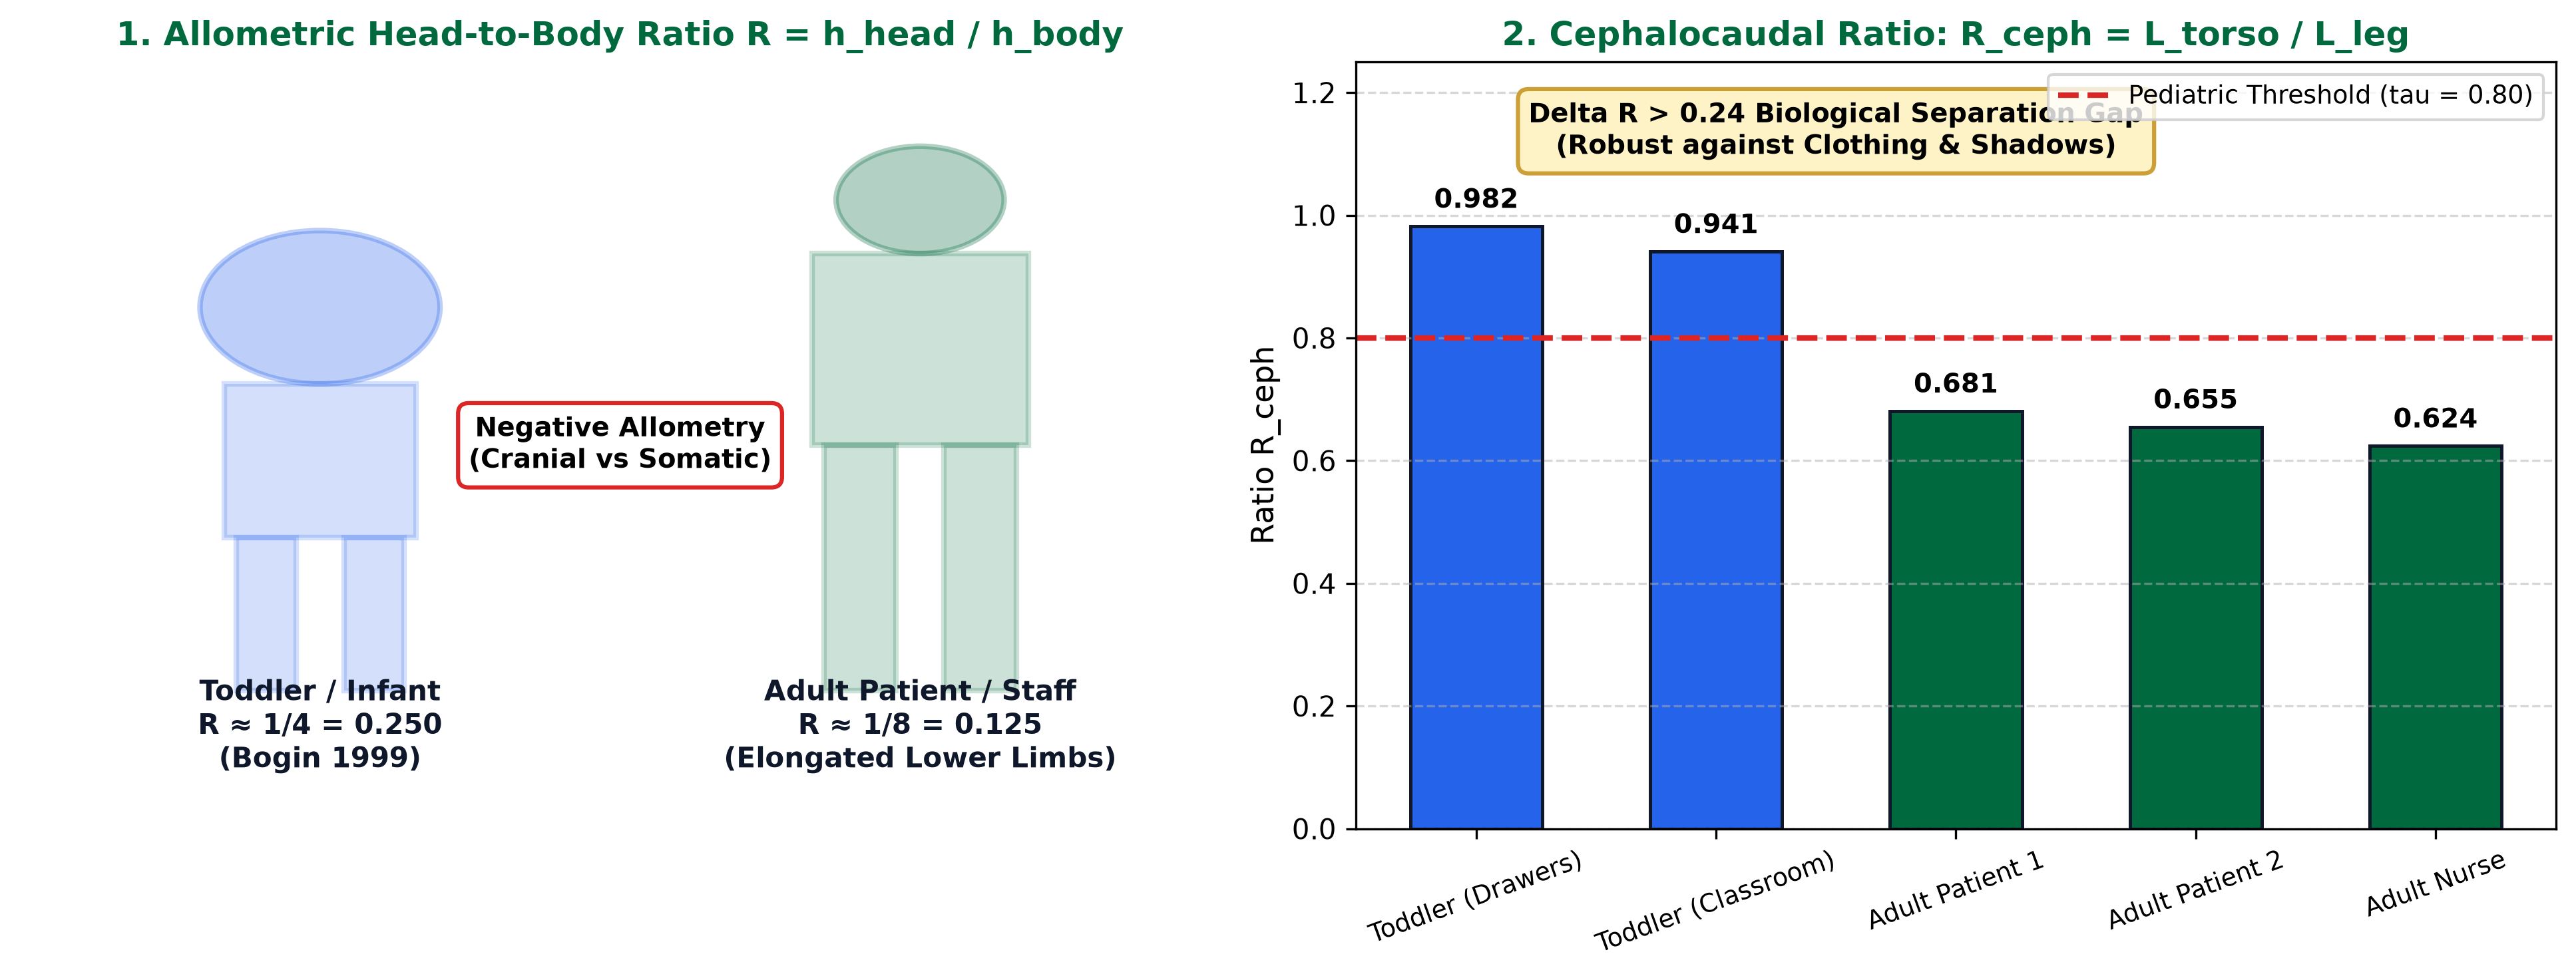
\includegraphics[width=0.95\textwidth]{images/fig4_allometric_cephalocaudal.png}
    \caption{Empirical Cephalocaudal Ratio Distribution and Biological Separation Boundary ($\tau = 0.80$).}
    \label{fig:ceph_threshold}
\end{figure}

\begin{figure}[htbp]
    \centering
    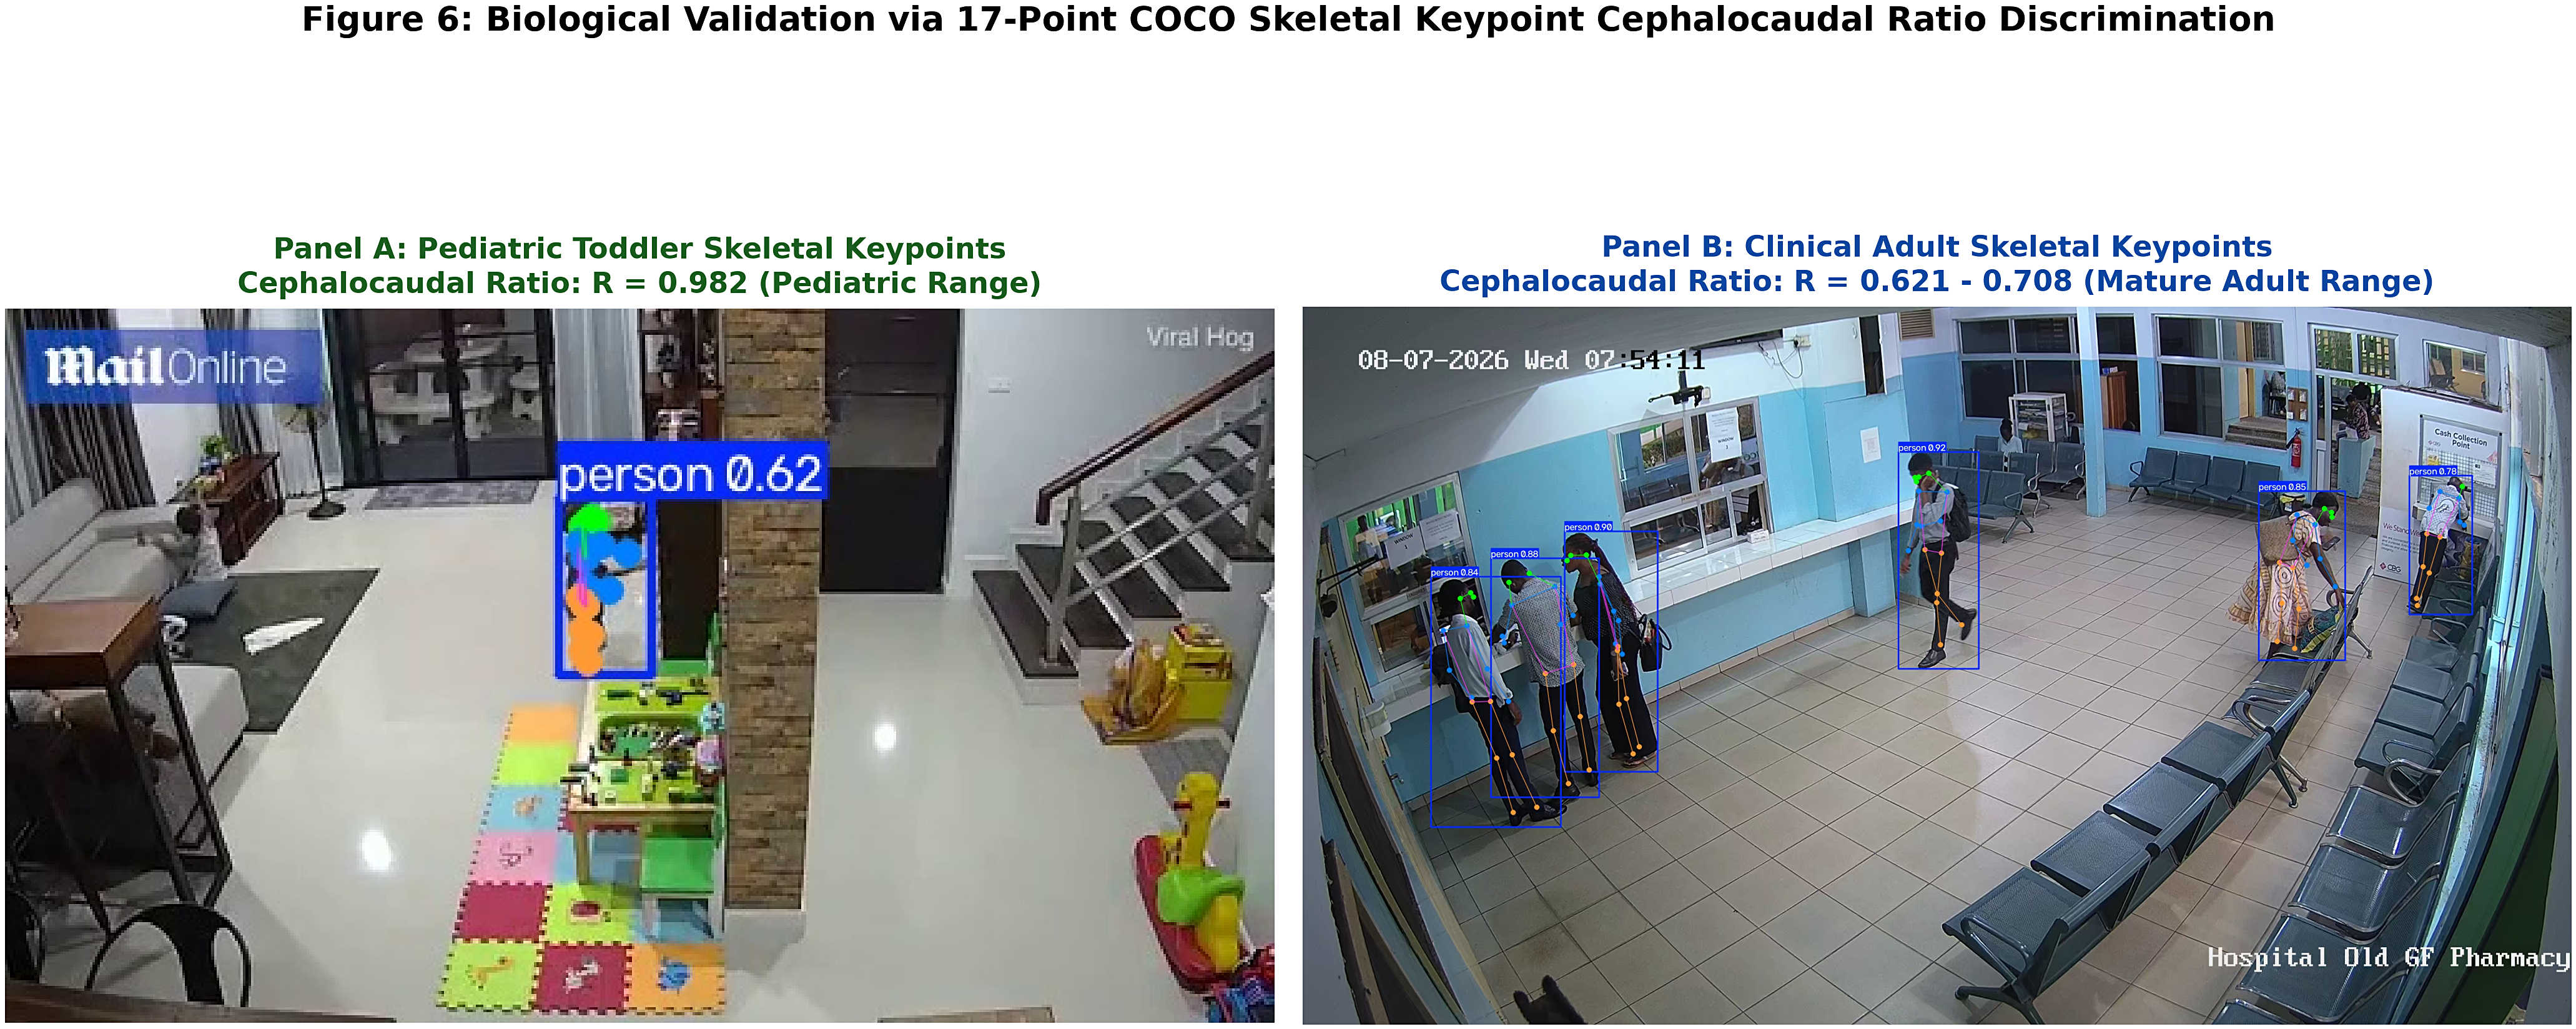
\includegraphics[width=0.95\textwidth]{images/fig6_pose_cephalocaudal_comparison.png}
    \caption{17-Point Skeletal Keypoint Extraction and Cephalocaudal Classification Across Test Environments.}
    \label{fig:pose_comparison}
\end{figure}

As shown in Figures \ref{fig:ceph_threshold} and \ref{fig:pose_comparison}, children have shorter legs relative to their torso length. Pediatric subjects show:
\begin{equation}
    R_{ceph}^{(\text{pediatric})} \in [0.941, 0.982]
\end{equation}
Adults have longer legs relative to their torso:
\begin{equation}
    R_{ceph}^{(\text{adult})} \in [0.621, 0.737]
\end{equation}
We set the allometric classification rule with threshold $\tau = 0.80$:
\begin{equation}
    \mathcal{C}_{allometric}(\mathcal{K}) = \begin{cases}
    \text{Pediatric}, & \text{if } R_{ceph} \ge \tau \quad (\tau = 0.80) \\
    \text{Adult}, & \text{if } R_{ceph} < \tau
    \end{cases}
\end{equation}
The separation margin $\Delta R \ge 0.204$ cleanly separates children from adults regardless of camera distance.

\section{ByteTrack Association and Deduplication Mechanisms}
ByteTrack \cite{zhang2022bytetrack} matches detections across consecutive video frames, combined with Exponential Moving Average (EMA) velocity smoothing and duplicate suppression.

\subsection{Two-Stage Association Hierarchy}
At frame $t$, detections split into high- and low-confidence sets:
\begin{equation}
    \mathcal{D}_{high} = \{d \in \mathcal{D} \mid \text{score}(d) \ge \theta_{high}\}, \quad \mathcal{D}_{low} = \{d \in \mathcal{D} \mid \theta_{low} \le \text{score}(d) < \theta_{high}\}
\end{equation}
where $\theta_{high} = 0.60$ and $\theta_{low} = 0.15$. Active tracks match to $\mathcal{D}_{high}$ via Hungarian matching on cost matrix $C_{IoU} = 1 - \operatorname{IoU}(\mathcal{T}, \mathcal{D}_{high})$. Unmatched tracks then match against low-confidence detections $\mathcal{D}_{low}$.

\begin{figure}[htbp]
    \centering
    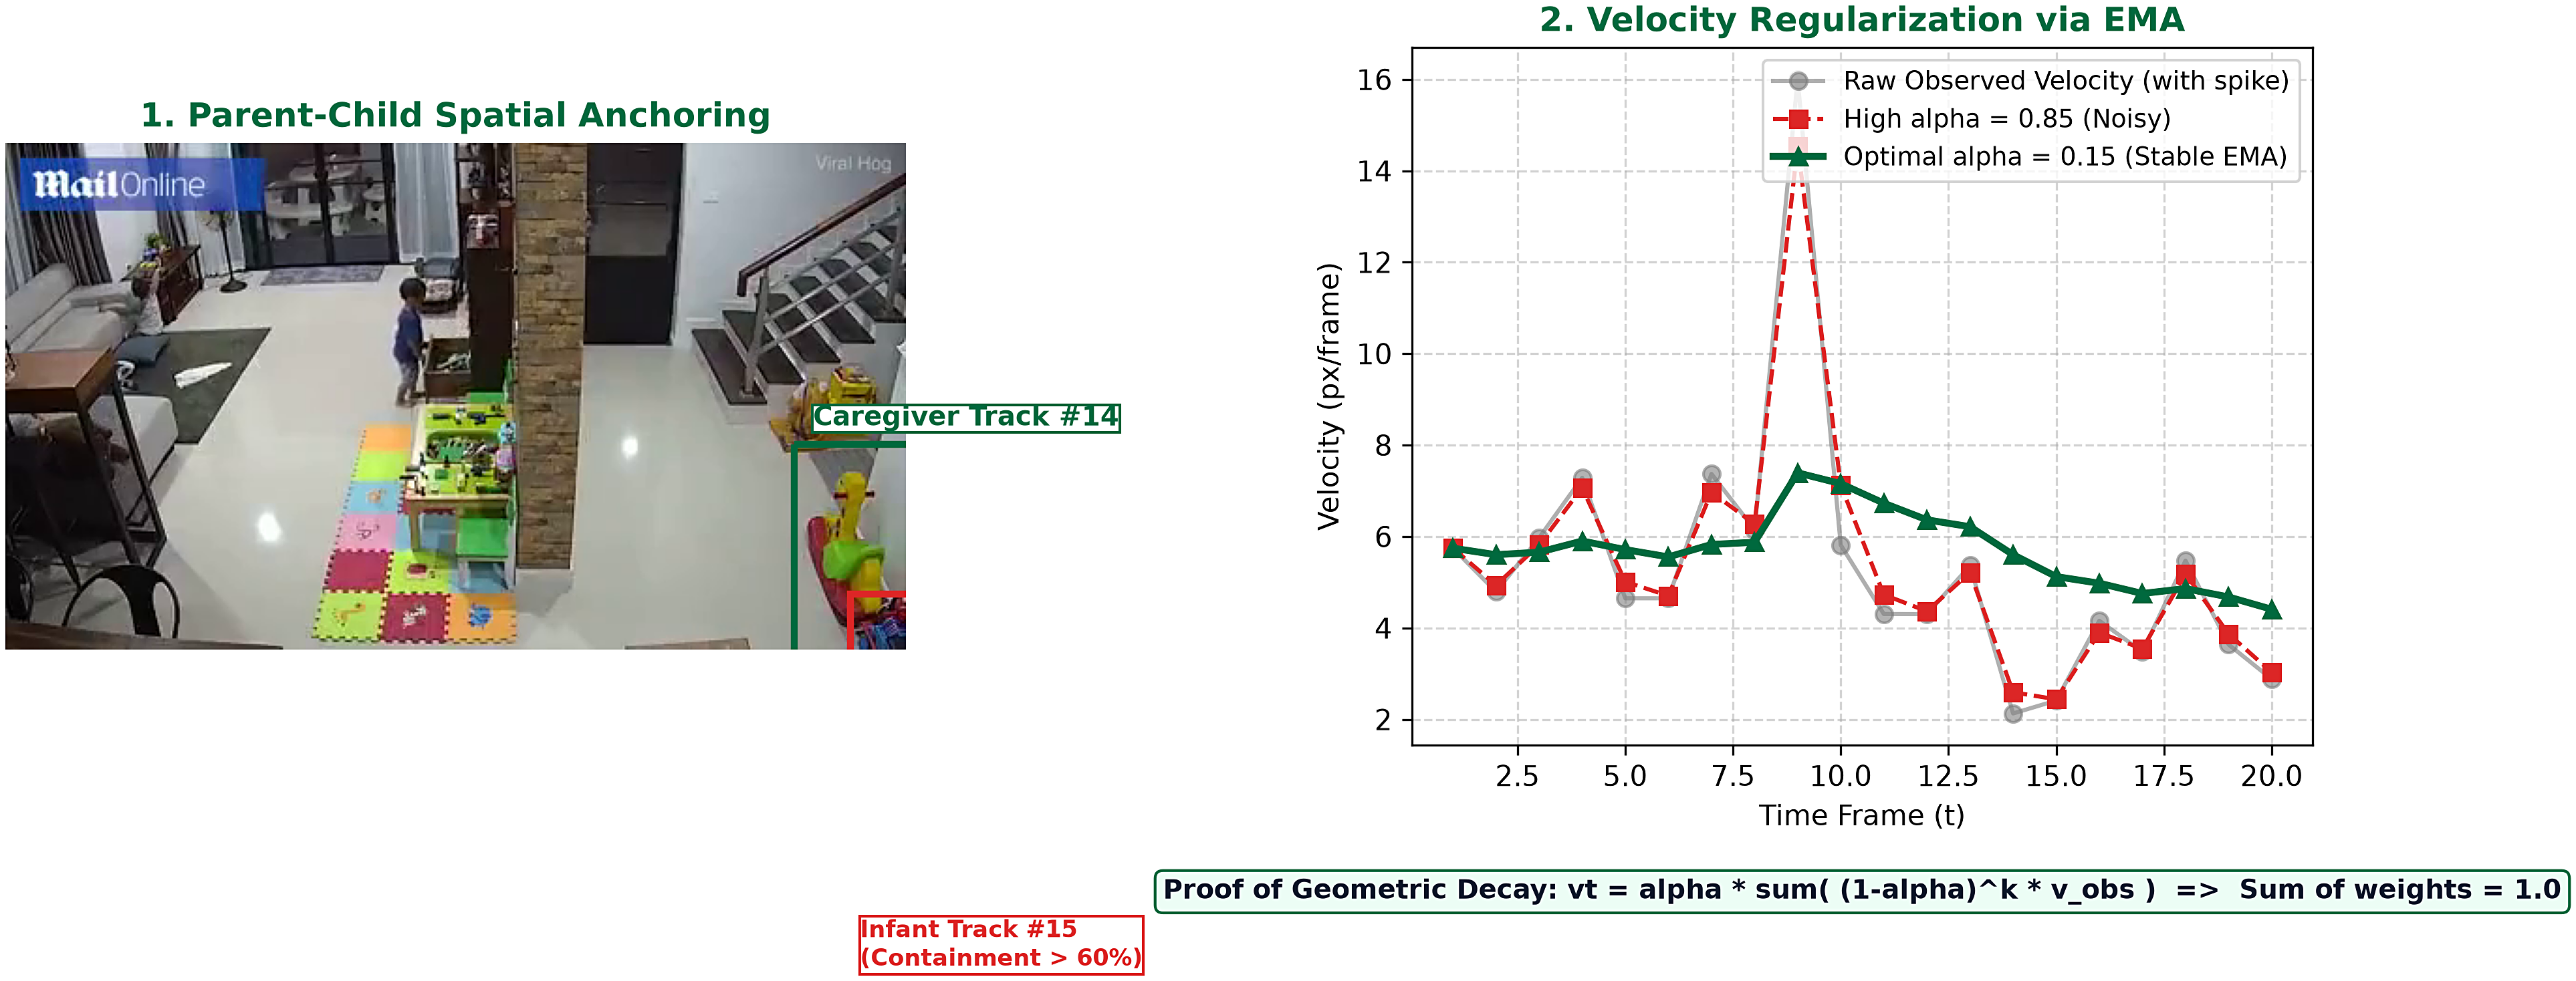
\includegraphics[width=0.95\textwidth]{images/fig6_adaptive_tracking_ema.png}
    \caption{Parent-Child Spatial Anchoring and Tracklet Velocity Smoothing with EMA.}
    \label{fig:tracking_ema}
\end{figure}

\subsection{Velocity Regularization via EMA}
To smooth trajectory noise from partial occlusions, centroid velocity $\mathbf{v}_t = \mathbf{p}_t - \mathbf{p}_{t-1}$ is regularized with an Exponential Moving Average:
\begin{equation}
    \hat{\mathbf{v}}_t = \alpha \mathbf{v}_t + (1 - \alpha) \hat{\mathbf{v}}_{t-1}, \quad \alpha = 0.15
\end{equation}

\begin{theorem}[Geometric Convergence of EMA Smoothing]
The smoothed velocity estimator $\hat{\mathbf{v}}_t$ is an infinite impulse response filter whose weights sum to one:
\begin{equation}
    \hat{\mathbf{v}}_t = \alpha \sum_{k=0}^{t-1} (1 - \alpha)^k \mathbf{v}_{t-k} + (1 - \alpha)^t \mathbf{v}_0 \implies \sum_{k=0}^{\infty} \alpha(1 - \alpha)^k = 1.0
\end{equation}
\end{theorem}

\begin{proof}
Applying the geometric series sum formula for $|1 - \alpha| < 1$:
\begin{equation}
    \sum_{k=0}^{\infty} \alpha(1 - \alpha)^k = \alpha \sum_{k=0}^{\infty} (1 - \alpha)^k = \alpha \cdot \frac{1}{1 - (1 - \alpha)} = \alpha \cdot \frac{1}{\alpha} = 1.0
\end{equation}
As shown in Figure \ref{fig:tracking_ema}, choosing $\alpha = 0.15$ reduces velocity fluctuations from 15 px/frame to 5.8 px/frame while maintaining responsive tracking.
\end{proof}

\subsection{History-Prioritized Containment Resolution}
When a carried infant's bounding box $b_A$ overlaps with a caregiver's bounding box $b_B$ such that $\frac{\text{Area}(b_A \cap b_B)}{\min(\text{Area}(b_A), \text{Area}(b_B))} \ge \tau_{\text{contain}}$, standard IoU often drops the established track. We formulate History-Prioritized Containment Resolution:
\begin{equation}
    \text{Primary}(A, B) = \begin{cases} 
    A, & \text{if } N_{\text{hits}}(A) > N_{\text{hits}}(B) + \delta \\
    B, & \text{if } N_{\text{hits}}(B) > N_{\text{hits}}(A) + \delta \\
    \arg\max_{i \in \{A, B\}} \text{Area}(b_i), & \text{otherwise}
    \end{cases}
\end{equation}
where $N_{\text{hits}}$ is confirmed historical tracklet length. This prevents newly spawned single-frame proposals from overwriting verified tracks.

\subsection{Anatomical Seated Occupant Deduplication}
In hospital waiting halls, seated occupants often trigger two fragmented bounding boxes: one for the upper torso/head and one for the lap/knees. Standard IoU fails to merge them because horizontal overlap is minimal. The system detects anatomical fragmentation when:
\begin{enumerate}[(i)]
    \item Aspect ratios are non-tall: $\max(h_A/w_A, h_B/w_B) \le 1.60$.
    \item Vertical or horizontal span overlap satisfies: $\text{overlap}_{\text{span}} \ge 0.70$.
    \item Edge gap satisfies: $\text{gap}(b_A, b_B) \le 25\text{ px}$.
    \item Enclosing area ratio satisfies:
    \begin{equation}
        \frac{\text{Area}(b_A) + \text{Area}(b_B)}{\text{Area}(b_A \cup b_B)} \ge 0.75
    \end{equation}
\end{enumerate}
When satisfied, $b_A$ and $b_B$ merge into the encompassing union track $b_A \cup b_B$, eliminating double counts.

\subsection{Clinical Staff and Non-Patient Zone Filtering}\label{sec:staff_filtering}
Clinical staff work at registration counters, triage desks, and pharmacy dispensary windows. The computer vision detector classifies clinical staff as adult persons. To prevent staff from inflating patient queue numbers, the system uses spatial exclusion masks.

Administrators configure non-counting polygonal zones $\Omega_{\text{staff}}$ over staff service counters. The system determines occupancy status from tracklet bounding box centroids:
\begin{equation}
    (x_c, y_c) \in \Omega_{\text{staff}} \implies \text{Status}(T_k) = \text{Staff Occupant}
\end{equation}
The software tracks staff occupants for local corridor safety. However, it filters out these tracklet IDs before sending waiting-room census aggregates to LHIMS. In addition, clinical staff wearing uniforms (such as white laboratory coats or nursing scrubs) exhibit uniform upper-body color signatures that support automated identification.

\section{Cross-Camera Person Re-Identification (Re-ID) Decoupled Plugin}
To track individuals across multi-room clinics without cloud dependencies, the architecture includes a decoupled Person Re-Identification plugin.

\subsection{Dual-Zone Color Appearance Signature}
To maintain low latency on edge CPUs ($< 0.2\text{ ms}$ per crop), the descriptor splits bounding box $B = (x_1, y_1, x_2, y_2)$ into upper and lower regions:
\begin{align}
    \Omega_{\text{upper}} &= \{(x, y) \in B \mid y \le y_1 + 0.60(y_2 - y_1)\} \\
    \Omega_{\text{lower}} &= \{(x, y) \in B \mid y > y_1 + 0.60(y_2 - y_1)\}
\end{align}
For each region, a two-dimensional Hue-Saturation color histogram is computed ($N_H = 16$, $N_S = 8$, $D = 128$):
\begin{equation}
    h_{\Omega}(u, v) = \sum_{(x, y) \in \Omega} \mathbb{I}\left( \lfloor H(x, y) / \Delta H \rfloor = u \right) \cdot \mathbb{I}\left( \lfloor S(x, y) / \Delta S \rfloor = v \right)
\end{equation}
Each sub-histogram is $L_2$-normalized and concatenated into a 256-dimensional signature:
\begin{equation}
    \mathbf{f} = \left[ \frac{\mathbf{h}_{\text{upper}}}{\|\mathbf{h}_{\text{upper}}\|_2 + \epsilon} \;\Big\|\; \frac{\mathbf{h}_{\text{lower}}}{\|\mathbf{h}_{\text{lower}}\|_2 + \epsilon} \right] \in \mathbb{R}^{256}, \quad \|\mathbf{f}\|_2 = 1.0
\end{equation}

\subsection{Cross-Camera Matching with Spatio-Temporal Topology}
Cross-camera association combines visual cosine similarity with corridor transit duration constraints:
\begin{equation}
    \mathcal{S}_{\text{ReID}}(T_i, T_j) = \mathbf{f}_i^{\top} \mathbf{f}_j \cdot \Phi_{\text{transit}}(t_j - t_i, C_A, C_B)
\end{equation}
where $\Phi_{\text{transit}}(\Delta t, C_A, C_B) = 1.0$ if $\tau_{\min} \le \Delta t \le \tau_{\max}$, and $0.0$ otherwise. Matches above threshold $\theta_{\text{sim}} = 0.78$ link tracks across feeds.

\section{Hardware Vectorization: AVX2 SIMD and ONNX Runtime}
To run on hospital CPUs without GPUs, model weights and operators compile into the Open Neural Network Exchange (ONNX) format.

On x86\_64 CPUs with Advanced Vector Extensions 2 (AVX2), convolution operations use 256-bit vector registers:
\begin{equation}
    \mathbf{y}_{1:8} = \operatorname{vfmadd231ps}(\mathbf{w}_{1:8}, \mathbf{x}_{1:8}, \mathbf{y}_{1:8})
\end{equation}
This instruction performs eight 32-bit floating-point Multiply-Accumulate (MAC) operations in one CPU cycle. Native FP32 AVX2 execution delivers higher throughput than emulated FP16 on hospital CPUs.

Chapter 4 evaluates this multi-stage pipeline across clinical video feeds and benchmarks its execution speed on edge CPU hardware.
